
\documentclass[sensors,article,submit,moreauthors,pdftex]{Definitions/mdpi}

\usepackage{graphicx,float}
\usepackage{amsmath,amssymb}
\usepackage{booktabs,array}
\usepackage{enumitem}
\usepackage{xurl}   % lets the repository URL break across lines


\providecommand{\TitleCitation}[1]{}
\providecommand{\AuthorCitation}[1]{}

% constants_base.tex -- written by analysis/build_paper_constants.py
% The main run's generated values that the manuscript quotes,
% resolved from constants.tex, constants_v10.tex, constants_thresholds.tex in
% analysis/main_run_constants/ (written by the main run's constants
% builder) and flattened to one definition each. Do not edit by hand.

\newcommand{\CatAdmitted}{753}
\newcommand{\CatBoostRtwo}{0.660}
\newcommand{\CatCandidates}{1,357}
\newcommand{\CollinearCut}{0.98}
\newcommand{\CountyScaleHi}{68}
\newcommand{\CountyScaleLo}{28}
\newcommand{\CountyScaleMed}{40}
\newcommand{\CoverageThreshold}{95}
\newcommand{\GateShapN}{20,000}
\newcommand{\HchoConRank}{196}
\newcommand{\HchoConSHAP}{0.004830}
\newcommand{\HchoDurCorr}{0.991}
\newcommand{\HchoDurRank}{1}
\newcommand{\HchoDurSHAP}{0.3407}
\newcommand{\HchoRatio}{70.5}
\newcommand{\MAEmodel}{1.033}
\newcommand{\MoranPerm}{999}
\newcommand{\NCEcandCols}{100}
\newcommand{\NCEcandSrc}{five}
\newcommand{\NCEcorr}{0.959}
\newcommand{\NCEmaxdiffMean}{$5.3\times10^{-10}$}
\newcommand{\NCEmeanRank}{133}
\newcommand{\NCEpctRank}{2}
\newcommand{\NCEratio}{20.3}
\newcommand{\Ncounties}{3{,}077}
\newcommand{\Nfeatpruned}{581}
\newcommand{\Nmodalities}{18}
\newcommand{\Nobs}{52{,}309}
\newcommand{\RawCorr}{+0.952}
\newcommand{\RefitDropMRtwo}{0.6695}
\newcommand{\RefitDropMeanRank}{29}
\newcommand{\RefitDropMeanSHAP}{0.03665}
\newcommand{\RefitDropRtwo}{0.6669}
\newcommand{\RefitFolds}{8}
\newcommand{\RefitFullMeanRank}{118}
\newcommand{\RefitFullMeanSHAP}{0.01238}
\newcommand{\RefitFullRtwo}{0.6680}
\newcommand{\RefitRecoveredPct}{10.2}
\newcommand{\Rtwo}{0.666}
\newcommand{\RtwoCIhi}{0.672}
\newcommand{\RtwoCIlo}{0.661}
\newcommand{\ShapCorr}{+0.022}
\newcommand{\StatFieldsTotal}{55}
\newcommand{\StrataTotal}{4}
\newcommand{\StrataWithCrossing}{2}
\newcommand{\YearEnd}{2019}
\newcommand{\YearStart}{2003}

% constants_results.tex -- written by analysis/build_paper_constants.py
% Do not edit by hand: rerun the script. Each block names the result
% file its values were read from.

% ---- baselines.json
\providecommand{\BlKnn}{}\renewcommand{\BlKnn}{0.642}

% ---- bracket_error.csv
\providecommand{\BrLowMAE}{}\renewcommand{\BrLowMAE}{6.56}
\providecommand{\BrMidMAE}{}\renewcommand{\BrMidMAE}{0.83}

% ---- spatial_holdout.json
\providecommand{\HoldStateRtwo}{}\renewcommand{\HoldStateRtwo}{0.509}

% ---- rank_stability.json
\providecommand{\LcTenRtwo}{}\renewcommand{\LcTenRtwo}{0.476}
\providecommand{\LcHalfRtwo}{}\renewcommand{\LcHalfRtwo}{0.649}
\providecommand{\LcFullRtwo}{}\renewcommand{\LcFullRtwo}{0.660}

% ---- null_skill.json
\providecommand{\NullSkillWithin}{}\renewcommand{\NullSkillWithin}{0.632}
\providecommand{\NullSkillBetween}{}\renewcommand{\NullSkillBetween}{$-$0.066}

% ---- temporal_validation.json
\providecommand{\LoyoMean}{}\renewcommand{\LoyoMean}{0.974}
\providecommand{\FwdMean}{}\renewcommand{\FwdMean}{0.940}

% ---- influence_drop.json
\providecommand{\InflDropN}{}\renewcommand{\InflDropN}{154}
\providecommand{\InflDropRtwo}{}\renewcommand{\InflDropRtwo}{0.761}
\providecommand{\InflOverlap}{}\renewcommand{\InflOverlap}{14}
\providecommand{\InflTopK}{}\renewcommand{\InflTopK}{15}

% ---- modality_arms.json
\providecommand{\ArmAllRtwo}{}\renewcommand{\ArmAllRtwo}{0.668}
\providecommand{\ArmAllN}{}\renewcommand{\ArmAllN}{581}

% ---- summary_statistic_census.json
\providecommand{\CensusMedianSpread}{}\renewcommand{\CensusMedianSpread}{3.4}

% ---- shap_dependence_check.json
\providecommand{\InvShapBackground}{}\renewcommand{\InvShapBackground}{500}

% ---- lifetime_literature_test.json
\providecommand{\LtSpecies}{}\renewcommand{\LtSpecies}{13}
\providecommand{\LtPairs}{}\renewcommand{\LtPairs}{20}
\providecommand{\LtRho}{}\renewcommand{\LtRho}{$-$0.42}
\providecommand{\LtPermP}{}\renewcommand{\LtPermP}{0.077}
\providecommand{\LtPerms}{}\renewcommand{\LtPerms}{20{,}000}
\providecommand{\LtCutoff}{}\renewcommand{\LtCutoff}{2}
\providecommand{\LtShortWins}{}\renewcommand{\LtShortWins}{5}
\providecommand{\LtShortN}{}\renewcommand{\LtShortN}{6}
\providecommand{\LtLongWins}{}\renewcommand{\LtLongWins}{2}
\providecommand{\LtLongN}{}\renewcommand{\LtLongN}{7}
\providecommand{\LtShortRatio}{}\renewcommand{\LtShortRatio}{2.42}
\providecommand{\LtLongRatio}{}\renewcommand{\LtLongRatio}{0.46}
\providecommand{\LtSweepN}{}\renewcommand{\LtSweepN}{7}
\providecommand{\LtSweepDirection}{}\renewcommand{\LtSweepDirection}{7}
\providecommand{\LtSweepSig}{}\renewcommand{\LtSweepSig}{1}
\providecommand{\LtJackLo}{}\renewcommand{\LtJackLo}{$-$0.55}
\providecommand{\LtJackHi}{}\renewcommand{\LtJackHi}{$-$0.30}
\providecommand{\LtValueDraws}{}\renewcommand{\LtValueDraws}{4{,}000}
\providecommand{\LtValueDex}{}\renewcommand{\LtValueDex}{0.5}
\providecommand{\LtValueNegative}{}\renewcommand{\LtValueNegative}{100}

% ---- turning_points.csv
\providecommand{\TpBoot}{}\renewcommand{\TpBoot}{5{,}000}
\providecommand{\TpStable}{}\renewcommand{\TpStable}{10}
\providecommand{\TpTotal}{}\renewcommand{\TpTotal}{11}
\providecommand{\TpDew}{}\renewcommand{\TpDew}{5.54}
\providecommand{\TpDewLo}{}\renewcommand{\TpDewLo}{5.51}
\providecommand{\TpDewHi}{}\renewcommand{\TpDewHi}{5.60}
\providecommand{\TpDewWidth}{}\renewcommand{\TpDewWidth}{0.3}
\providecommand{\TpDewAbove}{}\renewcommand{\TpDewAbove}{52.7}
\providecommand{\TpWet}{}\renewcommand{\TpWet}{7.41}
\providecommand{\TpWetLo}{}\renewcommand{\TpWetLo}{7.23}
\providecommand{\TpWetHi}{}\renewcommand{\TpWetHi}{7.48}
\providecommand{\TpWetWidth}{}\renewcommand{\TpWetWidth}{1.2}
\providecommand{\TpWetAbove}{}\renewcommand{\TpWetAbove}{38.5}
\providecommand{\TpNce}{}\renewcommand{\TpNce}{0.611}
\providecommand{\TpNceLo}{}\renewcommand{\TpNceLo}{0.608}
\providecommand{\TpNceHi}{}\renewcommand{\TpNceHi}{0.613}
\providecommand{\TpNceWidth}{}\renewcommand{\TpNceWidth}{0.5}
\providecommand{\TpNceAbove}{}\renewcommand{\TpNceAbove}{54.8}
\providecommand{\TpNceMean}{}\renewcommand{\TpNceMean}{0.492}
\providecommand{\TpNceMeanLo}{}\renewcommand{\TpNceMeanLo}{0.490}
\providecommand{\TpNceMeanHi}{}\renewcommand{\TpNceMeanHi}{0.498}
\providecommand{\TpNceMeanWidth}{}\renewcommand{\TpNceMeanWidth}{0.8}
\providecommand{\TpNceMeanAbove}{}\renewcommand{\TpNceMeanAbove}{65.4}
\providecommand{\TpLst}{}\renewcommand{\TpLst}{5.20}
\providecommand{\TpLstLo}{}\renewcommand{\TpLstLo}{5.23}
\providecommand{\TpLstHi}{}\renewcommand{\TpLstHi}{7.84}
\providecommand{\TpLstWidth}{}\renewcommand{\TpLstWidth}{13.2}
\providecommand{\TpLstAbove}{}\renewcommand{\TpLstAbove}{71.9}
\providecommand{\TpPm}{}\renewcommand{\TpPm}{0.51}
\providecommand{\TpPmLo}{}\renewcommand{\TpPmLo}{0.51}
\providecommand{\TpPmHi}{}\renewcommand{\TpPmHi}{0.87}
\providecommand{\TpPmWidth}{}\renewcommand{\TpPmWidth}{33.8}
\providecommand{\TpPmAbove}{}\renewcommand{\TpPmAbove}{88.0}
\providecommand{\TpTmin}{}\renewcommand{\TpTmin}{4.46}
\providecommand{\TpTminLo}{}\renewcommand{\TpTminLo}{4.28}
\providecommand{\TpTminHi}{}\renewcommand{\TpTminHi}{4.68}
\providecommand{\TpTminWidth}{}\renewcommand{\TpTminWidth}{1.7}
\providecommand{\TpTminAbove}{}\renewcommand{\TpTminAbove}{60.2}
\providecommand{\TpHcho}{}\renewcommand{\TpHcho}{27.5}
\providecommand{\TpHchoLo}{}\renewcommand{\TpHchoLo}{27.4}
\providecommand{\TpHchoHi}{}\renewcommand{\TpHchoHi}{27.8}
\providecommand{\TpHchoWidth}{}\renewcommand{\TpHchoWidth}{0.7}
\providecommand{\TpHchoAbove}{}\renewcommand{\TpHchoAbove}{43.3}
\providecommand{\TpRatio}{}\renewcommand{\TpRatio}{0.291}
\providecommand{\TpRatioLo}{}\renewcommand{\TpRatioLo}{0.288}
\providecommand{\TpRatioHi}{}\renewcommand{\TpRatioHi}{0.297}
\providecommand{\TpRatioWidth}{}\renewcommand{\TpRatioWidth}{1.3}
\providecommand{\TpRatioAbove}{}\renewcommand{\TpRatioAbove}{34.4}
\providecommand{\TpTripletWidthMax}{}\renewcommand{\TpTripletWidthMax}{1.2}

% ---- studyA_shap_ranking.csv (production ranking)
\providecommand{\CompN}{}\renewcommand{\CompN}{67}
\providecommand{\FamN}{}\renewcommand{\FamN}{10}
\providecommand{\FamOxVOCPct}{}\renewcommand{\FamOxVOCPct}{47.0}
\providecommand{\FamOxVOCn}{}\renewcommand{\FamOxVOCn}{7}
\providecommand{\FamSecondName}{}\renewcommand{\FamSecondName}{alkanes}
\providecommand{\FamSecondPct}{}\renewcommand{\FamSecondPct}{19.0}
\providecommand{\FamHchoPct}{}\renewcommand{\FamHchoPct}{45.4}
\providecommand{\FamHchoN}{}\renewcommand{\FamHchoN}{4}
\providecommand{\HchoNinetyRank}{}\renewcommand{\HchoNinetyRank}{4}
\providecommand{\PctRatio}{}\renewcommand{\PctRatio}{2.8}
\providecommand{\PctSpeciesN}{}\renewcommand{\PctSpeciesN}{8}
\providecommand{\PctSpeciesWins}{}\renewcommand{\PctSpeciesWins}{4}
\providecommand{\PctSpeciesMedRatio}{}\renewcommand{\PctSpeciesMedRatio}{1.03}
\providecommand{\PctPmLo}{}\renewcommand{\PctPmLo}{4.2}
\providecommand{\PctPmHi}{}\renewcommand{\PctPmHi}{13.3}
\providecommand{\PctRatioNoHcho}{}\renewcommand{\PctRatioNoHcho}{1.4}
\providecommand{\HchoPctRatio}{}\renewcommand{\HchoPctRatio}{2.4}
\providecommand{\SoilPninetyRank}{}\renewcommand{\SoilPninetyRank}{5}
\providecommand{\SoilMeanRank}{}\renewcommand{\SoilMeanRank}{6}
\providecommand{\SoilRatio}{}\renewcommand{\SoilRatio}{1.3}
\providecommand{\DPSummariesN}{}\renewcommand{\DPSummariesN}{7}
\providecommand{\DPMinRank}{}\renewcommand{\DPMinRank}{11}
\providecommand{\DPNextRank}{}\renewcommand{\DPNextRank}{189}
\providecommand{\DPMeanRank}{}\renewcommand{\DPMeanRank}{381}
\providecommand{\DPProfileRatio}{}\renewcommand{\DPProfileRatio}{11.0}

% ---- A_temp_strata.csv (main run)
\providecommand{\StrataCrossLo}{}\renewcommand{\StrataCrossLo}{5.57}
\providecommand{\StrataCrossHi}{}\renewcommand{\StrataCrossHi}{5.61}

% ---- A_modality_loo.csv (main run)
\providecommand{\LOOnModalities}{}\renewcommand{\LOOnModalities}{17}
\providecommand{\LOOcams}{}\renewcommand{\LOOcams}{$-$0.0080}
\providecommand{\LOOcamsN}{}\renewcommand{\LOOcamsN}{67}

% ---- null_crossing.json
\providecommand{\NullCrossTotal}{}\renewcommand{\NullCrossTotal}{440}
\providecommand{\NullCrossPasses}{}\renewcommand{\NullCrossPasses}{0}
\providecommand{\NullCrossDraws}{}\renewcommand{\NullCrossDraws}{40}
\providecommand{\NullCrossBoot}{}\renewcommand{\NullCrossBoot}{120}
\providecommand{\NullCrossShifted}{}\renewcommand{\NullCrossShifted}{0}

% ---- perturbation_thresholds.csv
\providecommand{\PertOneMed}{}\renewcommand{\PertOneMed}{0.06}
\providecommand{\PertOneMax}{}\renewcommand{\PertOneMax}{0.21}
\providecommand{\PertTwoMed}{}\renewcommand{\PertTwoMed}{0.13}
\providecommand{\PertTwoMax}{}\renewcommand{\PertTwoMax}{0.28}
\providecommand{\PertFiveMed}{}\renewcommand{\PertFiveMed}{0.24}
\providecommand{\PertFiveMax}{}\renewcommand{\PertFiveMax}{0.79}
\providecommand{\PertTenMed}{}\renewcommand{\PertTenMed}{0.50}
\providecommand{\PertTenMax}{}\renewcommand{\PertTenMax}{1.90}
\providecommand{\PertDraws}{}\renewcommand{\PertDraws}{25}

% ---- threshold_regional_invariance_all.json
\providecommand{\RegMedCut}{}\renewcommand{\RegMedCut}{90.1}
\providecommand{\RegMedWest}{}\renewcommand{\RegMedWest}{9{,}993}
\providecommand{\RegMedEast}{}\renewcommand{\RegMedEast}{10{,}002}
\providecommand{\RegMedMatched}{}\renewcommand{\RegMedMatched}{19{,}995}
\providecommand{\RegMedDew}{}\renewcommand{\RegMedDew}{0.7}
\providecommand{\RegMedDewAbs}{}\renewcommand{\RegMedDewAbs}{0.18}
\providecommand{\RegMedWet}{}\renewcommand{\RegMedWet}{1.1}
\providecommand{\RegMedWetAbs}{}\renewcommand{\RegMedWetAbs}{0.23}
\providecommand{\RegMedNce}{}\renewcommand{\RegMedNce}{0.6}
\providecommand{\RegMedNceAbs}{}\renewcommand{\RegMedNceAbs}{0.006}
\providecommand{\RegMedLst}{}\renewcommand{\RegMedLst}{5.5}
\providecommand{\RegMedPm}{}\renewcommand{\RegMedPm}{38.5}
\providecommand{\RegMedRatio}{}\renewcommand{\RegMedRatio}{24.8}
\providecommand{\RegMedWetHot}{}\renewcommand{\RegMedWetHot}{3.4}
\providecommand{\RegMedTmin}{}\renewcommand{\RegMedTmin}{0.2}
\providecommand{\RegMedTripletMax}{}\renewcommand{\RegMedTripletMax}{1.1}

% ---- threshold_regional_invariance_100W_all.json
\providecommand{\RegMerCut}{}\renewcommand{\RegMerCut}{100}
\providecommand{\RegMerWest}{}\renewcommand{\RegMerWest}{3{,}782}
\providecommand{\RegMerEast}{}\renewcommand{\RegMerEast}{16{,}213}
\providecommand{\RegMerMatched}{}\renewcommand{\RegMerMatched}{19{,}995}
\providecommand{\RegMerDew}{}\renewcommand{\RegMerDew}{1.2}
\providecommand{\RegMerDewAbs}{}\renewcommand{\RegMerDewAbs}{0.32}
\providecommand{\RegMerWet}{}\renewcommand{\RegMerWet}{1.0}
\providecommand{\RegMerWetAbs}{}\renewcommand{\RegMerWetAbs}{0.22}
\providecommand{\RegMerNce}{}\renewcommand{\RegMerNce}{1.7}
\providecommand{\RegMerNceAbs}{}\renewcommand{\RegMerNceAbs}{0.015}
\providecommand{\RegMerLst}{}\renewcommand{\RegMerLst}{10.1}
\providecommand{\RegMerPm}{}\renewcommand{\RegMerPm}{30.3}
\providecommand{\RegMerRatio}{}\renewcommand{\RegMerRatio}{4.3}
\providecommand{\RegMerWetHot}{}\renewcommand{\RegMerWetHot}{2.6}
\providecommand{\RegMerTmin}{}\renewcommand{\RegMerTmin}{2.6}
\providecommand{\RegMerTripletMax}{}\renewcommand{\RegMerTripletMax}{1.7}

% ---- residual_social_determinants.json
\providecommand{\ResSdohRtwo}{}\renewcommand{\ResSdohRtwo}{0.44}
\providecommand{\ResEnvRtwo}{}\renewcommand{\ResEnvRtwo}{$-$0.17}
\providecommand{\ResSdohN}{}\renewcommand{\ResSdohN}{314}
\providecommand{\ResEnvN}{}\renewcommand{\ResEnvN}{581}
\providecommand{\ResSD}{}\renewcommand{\ResSD}{1.38}
\providecommand{\ResMissN}{}\renewcommand{\ResMissN}{52}
\providecommand{\ResMissYears}{}\renewcommand{\ResMissYears}{3}
\providecommand{\ResPovRho}{}\renewcommand{\ResPovRho}{$-$0.34}
\providecommand{\ResPovPct}{}\renewcommand{\ResPovPct}{90}
\providecommand{\ResIncRho}{}\renewcommand{\ResIncRho}{0.35}
\providecommand{\ResIncPct}{}\renewcommand{\ResIncPct}{17}
\providecommand{\ResUnempRho}{}\renewcommand{\ResUnempRho}{$-$0.29}
\providecommand{\ResUnempPct}{}\renewcommand{\ResUnempPct}{93}
\providecommand{\ResUninsRho}{}\renewcommand{\ResUninsRho}{$-$0.19}
\providecommand{\ResUninsPct}{}\renewcommand{\ResUninsPct}{80}
\providecommand{\ResBachRho}{}\renewcommand{\ResBachRho}{0.33}
\providecommand{\ResBachPct}{}\renewcommand{\ResBachPct}{34}
\providecommand{\ResDisRho}{}\renewcommand{\ResDisRho}{$-$0.30}
\providecommand{\ResDisPct}{}\renewcommand{\ResDisPct}{56}
\providecommand{\ResHolmMax}{}\renewcommand{\ResHolmMax}{$2.4\times10^{-26}$}
\providecommand{\ResAbsRhoLo}{}\renewcommand{\ResAbsRhoLo}{0.19}
\providecommand{\ResAbsRhoHi}{}\renewcommand{\ResAbsRhoHi}{0.35}
\providecommand{\ResSdohYearLo}{}\renewcommand{\ResSdohYearLo}{2009}
\providecommand{\ResSdohYearHi}{}\renewcommand{\ResSdohYearHi}{2019}
\providecommand{\ResAcsN}{}\renewcommand{\ResAcsN}{274}
\providecommand{\ResNoChrN}{}\renewcommand{\ResNoChrN}{298}
\providecommand{\ResNoChrRtwo}{}\renewcommand{\ResNoChrRtwo}{0.43}
\providecommand{\ResAcsRtwo}{}\renewcommand{\ResAcsRtwo}{0.43}

% ---- residual_spatial_structure.json
\providecommand{\ResMoranI}{}\renewcommand{\ResMoranI}{0.036}
\providecommand{\ResMoranP}{}\renewcommand{\ResMoranP}{0.007}
\providecommand{\ResMoranOutcome}{}\renewcommand{\ResMoranOutcome}{0.68}

% ---- formaldehyde_drop.json
\providecommand{\HchoDropFullRtwo}{}\renewcommand{\HchoDropFullRtwo}{0.6680}
\providecommand{\HchoDropOneRtwo}{}\renewcommand{\HchoDropOneRtwo}{0.6657}
\providecommand{\HchoDropBothRtwo}{}\renewcommand{\HchoDropBothRtwo}{0.6635}
\providecommand{\HchoDropInheritPct}{}\renewcommand{\HchoDropInheritPct}{72}
\providecommand{\HchoDropShapN}{}\renewcommand{\HchoDropShapN}{3{,}000}
\providecommand{\HchoDropShapBg}{}\renewcommand{\HchoDropShapBg}{120}
\providecommand{\HchoColRankWith}{}\renewcommand{\HchoColRankWith}{95}
\providecommand{\HchoColRankWithout}{}\renewcommand{\HchoColRankWithout}{3}
\providecommand{\HchoDropBothCost}{}\renewcommand{\HchoDropBothCost}{0.004}
\providecommand{\HchoSurfRankWith}{}\renewcommand{\HchoSurfRankWith}{161}
\providecommand{\HchoSurfRankWithout}{}\renewcommand{\HchoSurfRankWithout}{22}

% ---- studyA_oof_predictions.csv
\providecommand{\PredMean}{}\renewcommand{\PredMean}{77.2}

% ---- nce_refit.json (refit protocol)
\providecommand{\RefitTrees}{}\renewcommand{\RefitTrees}{1{,}200}
\providecommand{\RefitLR}{}\renewcommand{\RefitLR}{0.03}
\providecommand{\RefitDepth}{}\renewcommand{\RefitDepth}{8}
\providecommand{\RefitShapN}{}\renewcommand{\RefitShapN}{20{,}000}
\providecommand{\RefitShapBg}{}\renewcommand{\RefitShapBg}{500}
\providecommand{\RefitFullTailSHAP}{}\renewcommand{\RefitFullTailSHAP}{0.2381}

% ---- library_version_sensitivity.json
\providecommand{\VerPython}{}\renewcommand{\VerPython}{3.11.13}
\providecommand{\VerXgb}{}\renewcommand{\VerXgb}{3.0.2}
\providecommand{\VerShap}{}\renewcommand{\VerShap}{0.48.0}
\providecommand{\VerSklearn}{}\renewcommand{\VerSklearn}{1.7.1}
\providecommand{\VerNumpy}{}\renewcommand{\VerNumpy}{2.2.6}
\providecommand{\VerPandas}{}\renewcommand{\VerPandas}{2.2.3}
\providecommand{\VerScipy}{}\renewcommand{\VerScipy}{1.16.1}
\providecommand{\VerCatboost}{}\renewcommand{\VerCatboost}{1.2.8}


\firstpage{1}
\makeatletter\setcounter{page}{\@firstpage}\makeatother

\pubvolume{1}
\issuenum{1}
\articlenumber{0}
\pubyear{2026}
\copyrightyear{2026}
%\externaleditor{Firstname Lastname}
\datereceived{ }
\daterevised{ }
\dateaccepted{ }
\datepublished{ }

\newcommand{\orcidauthorA}{0009-0006-0330-8993}
\newcommand{\orcidauthorB}{0000-0003-4265-9543}
\newcommand{\orcidauthorC}{0000-0002-5910-0183}
\newcommand{\orcidauthorD}{0000-0002-0126-218X}
\newcommand{\orcidauthorE}{0009-0007-7357-1479}
\newcommand{\orcidauthorF}{0009-0008-9351-3644}
\newcommand{\orcidauthorG}{0000-0003-2688-648X}

\Title{How Long, Not How Much: Summarising Satellite and Gridded Data Reorders Machine Learning Predictors of U.S. County Life Expectancy}

\TitleCitation{How Long, Not How Much: Summarising Satellite and Gridded Data Reorders Machine Learning Predictors of U.S. County Life Expectancy}



\Author{Faiz Ahmad$^{1}$\orcidA{},
  David J.\ Lary$^{1,*}$\orcidB{},
  Shisir Ruwali$^{1}$\orcidE{},
  Samyak Shrestha$^{1}$\orcidF{},
  Adam Aker$^{1}$\orcidD{},
  John Waczak$^{1}$\orcidC{},
  Md Shaid Hasan Niloy$^{1}$,
  Rittik Patra$^{1}$,
  Tunde Dare Awoyinka$^{1}$,
  Lakitha Omal Harindha Wijeratne$^{1}$\orcidG{}
  and Mazhar Iqbal$^{1}$}

\AuthorNames{Faiz Ahmad, David J. Lary, Shisir Ruwali, Samyak Shrestha,
             Adam Aker, John Waczak, Md Shaid Hasan Niloy, Rittik Patra,
             Tunde Dare Awoyinka, Lakitha Omal Harindha Wijeratne and
             Mazhar Iqbal}

\address{%
$^{1}$ \quad Department of Physics, The University of Texas at Dallas,
  800 W Campbell Rd, Richardson, TX 75080, USA;
  faiz.ahmad@utdallas.edu (F.A.); david.lary@utdallas.edu (D.J.L.);
  shisir.ruwali@utdallas.edu (S.R.); samyak.shrestha@utdallas.edu (S.S.);
  adam.r.a1@utdallas.edu (A.A.); john.waczak@utdallas.edu (J.W.);
  MdShaidHasan.Niloy@utdallas.edu (M.S.H.N.); Rittik.Patra@utdallas.edu (R.P.);
  Tunde.Awoyinka@utdallas.edu (T.D.A.); lhw150030@utdallas.edu (L.O.H.W.);
  Mazhar.Iqbal@utdallas.edu (M.I.)}

\corres{Correspondence: david.lary@utdallas.edu (D.J.L.)}


%% ==========================================================================
%%  ABSTRACT  (MDPI limit: 200 words; no abbreviations by house rule)
%% ==========================================================================
\abstract{%
Life expectancy differs by more than twenty years between United States
counties, and part of that gap is environmental. Global datasets provide data to
map the heat, air and land around every county, and researchers often naturally ask
which conditions go with longer lives. However, the answer depends on a step
few question: how a year of measurements is boiled down to one number. For
formaldehyde, an air pollutant, the computer rewarded how long, not how much:
the fraction of the year that levels stayed high counted far more than the
yearly average. A machine-learning model given yearly summaries for
\Ncounties{} counties over \YearStart{}--\YearEnd{} explained \Rtwo{} of the
variation in life expectancy among unseen counties. Its top-ranked input, the
time formaldehyde spent above the upper quartile of county averages, carried
\HchoRatio{} times the attribution of formaldehyde's average. For other
quantities, the most and least attributed summaries of each differed by
a median factor of \CensusMedianSpread{}. Refitted without formaldehyde's
time-above-level summaries, the model lost only \HchoDropBothCost{} of
explained variation and moved attribution to the averages. Its errors followed
social conditions it was never shown (\ResSdohRtwo{} of error variation).
Such rankings reflect how data were summarised and are not evidence of cause.
}

\keyword{satellite remote sensing; atmospheric reanalysis; summary statistics;
Shapley additive explanations; explainable machine learning; formaldehyde; atmospheric
lifetime; night cooling efficiency; wet-bulb temperature; social determinants
of health}

%% Highlights not rendered (owner ruling 2026-11-13: no bulleted list at the start of the paper). %\addhighlights{%
%\minisec{What are the main findings?}
%\begin{itemize}[nosep]
%\item With the data held fixed, formaldehyde ranked first as time above the national 75th percentile and \HchoConRank{}th as its annual mean, a \HchoRatio{}-fold gap in attribution. Two night cooling efficiency formulas from one land-surface temperature product differed \NCEratio{}-fold.
%\item Removing both formaldehyde durations lowered the coefficient of determination by only \HchoDropBothCost{}, and across \LtSpecies{} species the advantage of duration over the mean tended to fall with atmospheric lifetime (one-sided $p$ = \LtPermP{}).
%\end{itemize}
%\minisec{What are the implications of the main findings?}
%\begin{itemize}[nosep]
%\item Studies that rank satellite-derived environmental factors should report the summary of each field as a choice, match it to the timescale of the process, and test a leading rank with a drop-one refit.
%\item The model's error follows socioeconomic conditions it never saw and is largest in the shortest-lived counties, so use elsewhere, for example toward Sustainable Development Goal target 3.9, needs recalibration against local mortality data first.
%\end{itemize}
%}

%% ======================================================================
\begin{document}

%% ======================================================================
\section{Introduction}
\label{sec:intro}

Life expectancy at birth summarises in one number the combined influence of
environmental stress, disease burden, economic deprivation, and behavioural
risk~\cite{Murray2013, Chetty2016}. In 2014 it differed across United States counties by
more than twenty years~\cite{DwyerLindgren2017}. Part of that gap is
environmental: falling fine particulate matter was associated with longer life
expectancy in metropolitan counties~\cite{Pope2009}. Above its lowest
observed level, the pollutant was estimated to shorten life expectancy at
national and county scale~\cite{Bennett2019}.

Satellites and reanalyses (weather and chemistry models constrained by
observations) record the physical environment of every county through the year. They
sample its land-surface temperature by day and by night, the trace gases above
it, the moisture of its air, and its soils, water, and vegetation. Machine
learning models fed with such data predict population health outcomes, from neighbourhood obesity prevalence~\cite{Maharana2018} and
county mortality~\cite{Levy2021} to county life
expectancy~\cite{Ruwali2026multi, Ahmad2026night}. Attribution methods such as
SHapley Additive exPlanations (SHAP) divide each
prediction among the inputs and so name the measurements the prediction leans
on~\cite{Lundberg2017, Lundberg2020}. Such attribution has become a common way
to draw conclusions from remote-sensing models~\cite{Hohl2024}.

Between the satellite and the model sits a choice of summary. A sensor delivers a field, thousands of pixels per county and dozens of
overpasses per year, but the model needs one number per county and year. Cohort
studies of chronic exposure use the annual mean~\cite{Pope2020, Di2017, Burnett2018}. Yet the
annual mean records how much, not how long: two counties with the same mean
can differ, one passing through frequent high episodes, the other sitting at a
steady moderate level. Exposure science has
long known that the metric chosen for one pollutant changes the health
association estimated with it~\cite{Ozkaynak2013, Dionisio2016}. The daily
peak, the 24-hour mean, and the daytime or night-time average of one pollutant
carried different associations~\cite{Darrow2009}. The intensity and the
duration of a heat wave modified mortality separately~\cite{Anderson2010}.
In satellite thermal images of Paris during the 2003 heat wave, only the
minimum surface temperature, not the maximum, mean, or daily range, was
associated with deaths of older people~\cite{Laaidi2011}.
Over years rather than days, the summer standard deviation of temperature, not
only its mean, was associated with the survival of older
adults~\cite{Zanobetti2012, Shi2015}.
Air-quality and climate assessments already count the days above a level or
sum the excess over it, for ozone~\cite{Fleming2018} and for temperature
extremes~\cite{Zhang2011}. Land-cover mapping likewise feeds a classifier
several summaries of each pixel's time
series~\cite{Pflugmacher2019}.

Our earlier county studies ranked three environmental measures among the
leading correlates of county life expectancy and cardiovascular mortality.
They were night-time thermal
patterns~\cite{Ahmad2026night}, formaldehyde duration (the time spent above a
reference level)~\cite{Shrestha2026exp, Shrestha2026cvd}, and wet-bulb
temperature (a joint measure of heat and
humidity)~\cite{Ruwali2026multi, Shrestha2026cvd}. The night-time result agrees with evidence that hot nights carry
their own mortality risk~\cite{He2022}.

Machine learning studies that rank satellite inputs by attribution have not, to
our knowledge, treated the summary as a variable. Yet a model offered several
summaries of one field can route its prediction through whichever it finds
convenient, and attribution then names that one as important. Attribution adds
its own dependence on how it is divided among correlated
inputs~\cite{Strobl2008, Kumar2020, Janzing2020}. Many models can fit the
same data almost equally well yet rank the inputs
differently~\cite{Breiman2001two, Fisher2019}. How much of our earlier
rankings belongs to the way each field was summarised remains untested.

This paper treats the summary statistic as an experimental variable in one
gradient-boosted ensemble of decision trees~\cite{Friedman2001}. The ensemble predicts small-area estimates of life expectancy at birth~\cite{DwyerLindgren2022}, both sexes combined, in
counties of the contiguous United States from \YearStart{} to \YearEnd{}. The
fields include trace gases from the reanalysis of the Copernicus Atmosphere Monitoring Service
(CAMS)~\cite{Inness2019}, taken from the county extraction of our
earlier studies~\cite{Ruwali2026multi, Shrestha2026exp}, and land-surface temperature
from the Moderate Resolution Imaging Spectroradiometer
(MODIS)~\cite{Wan2014}. Dew
point comes from the station-based climate grid of the Parameter-elevation Regressions on Independent Slopes
Model (PRISM)~\cite{Daly2008, Daly2015}. In CAMS, formaldehyde is a model
field, not a satellite retrieval. Chemistry gives
a reason to expect the summary to matter. A gas destroyed within hours rises
and falls with its sources and reaches people as episodes; a gas that persists
for weeks mixes into a regional background~\cite{Seinfeld2016}. Duration may
suit the first, and the annual mean the second.

We ask four questions about how attribution behaves, not how large any
environmental effect is. First, with the data held fixed, how far does the
summary chosen for a field move the attribution a model gives it, and do
refits without the leading summary lose skill or only move attribution?
Second, which chemical families (groups of related species) carry the
attribution, and does atmospheric lifetime track whether the model favours
duration or the annual mean? Third, do the values at which a
variable's attribution changes sign, its turning points, meet a stability
criterion (found in most resamples, narrowly
located, and agreeing with the full sample)? Do they survive added noise and a climatic split of
the country? Fourth, where does a model built only
from satellite and gridded data err, and do socioeconomic variables it never saw
explain that error?

Formaldehyde's leading duration, a case chosen post hoc, carried \HchoRatio{} times
the attribution of its annual mean, perhaps partly by how duration is defined or by grid cells wider than most counties. Drop-one refits of two fields, each
without its leading summary, left skill almost unchanged but changed
the ranking. Formaldehyde carried \FamHchoPct{}\% (no interval) of the attribution given to
atmospheric composition, and duration's advantage over the mean tended to fall with
atmospheric lifetime (one-sided permutation $p$ = \LtPermP{}, \LtSpecies{} species). Of
\TpTotal{} candidate turning points, \TpStable{} met the stability criterion, on intervals likely too narrow.
Within one fitted model, the dew-point, wet-bulb, and night-cooling points moved by at most
\RegMerTripletMax{}\% of their range between the drier west and humid east, two exceeding their resampling-interval widths. Satellite-derived fine particulate matter, which passed only formally, moved by \RegMerPm{}\% of its range.
Socioeconomic variables the model never saw predicted its error (coefficient
of determination \ResSdohRtwo{}), though part may enter through the county covariates behind the life-expectancy estimates. For remote sensing, the summary statistic
is a design choice, to be reported with
the product and tested with a drop-one refit.

%% ======================================================================
\section{Materials and Methods}
\label{sec:methods}

\subsection{Study Design}
\label{ssec:m_design}
In this ecological panel study we linked satellite-derived and gridded environmental measurements to life
expectancy across \Ncounties{} counties of the contiguous United States from
\YearStart{} to \YearEnd{}, giving \Nobs{} county-year observations
(Figure~\ref{fig:method}). The analysis is predictive: the questions
concern how a fitted model's attribution behaves, not how large any environmental effect is. Counties
entered only if all seventeen years of the study window were present, so the
panel was balanced and every county had equal weight
(Section~\ref{ssec:d_limits}).
No census, demographic, economic, or clinical variable entered the model
directly. Some gridded inputs nonetheless record human presence: night-time
lights, and the Global Human Modification index, whose inputs include
population density~\cite{Kennedy2019}. An environmental column correlated with the
socioeconomic surface of the same counties can carry socioeconomic as well as
environmental information. Its attribution therefore need not equal its
environmental share: socioeconomic signal can inflate it, or offset it where
the two act in opposite directions. Keeping the socioeconomic layer out also lets it serve afterwards as an
independent test of where the model errs (Section~\ref{ssec:m_sdoh}). The earlier county
study of formaldehyde duration showed that its association with life
expectancy persists after adjustment for poverty, education, and
smoking~\cite{Shrestha2026exp}; we take that result as given.

\begin{figure}[H]
\centering
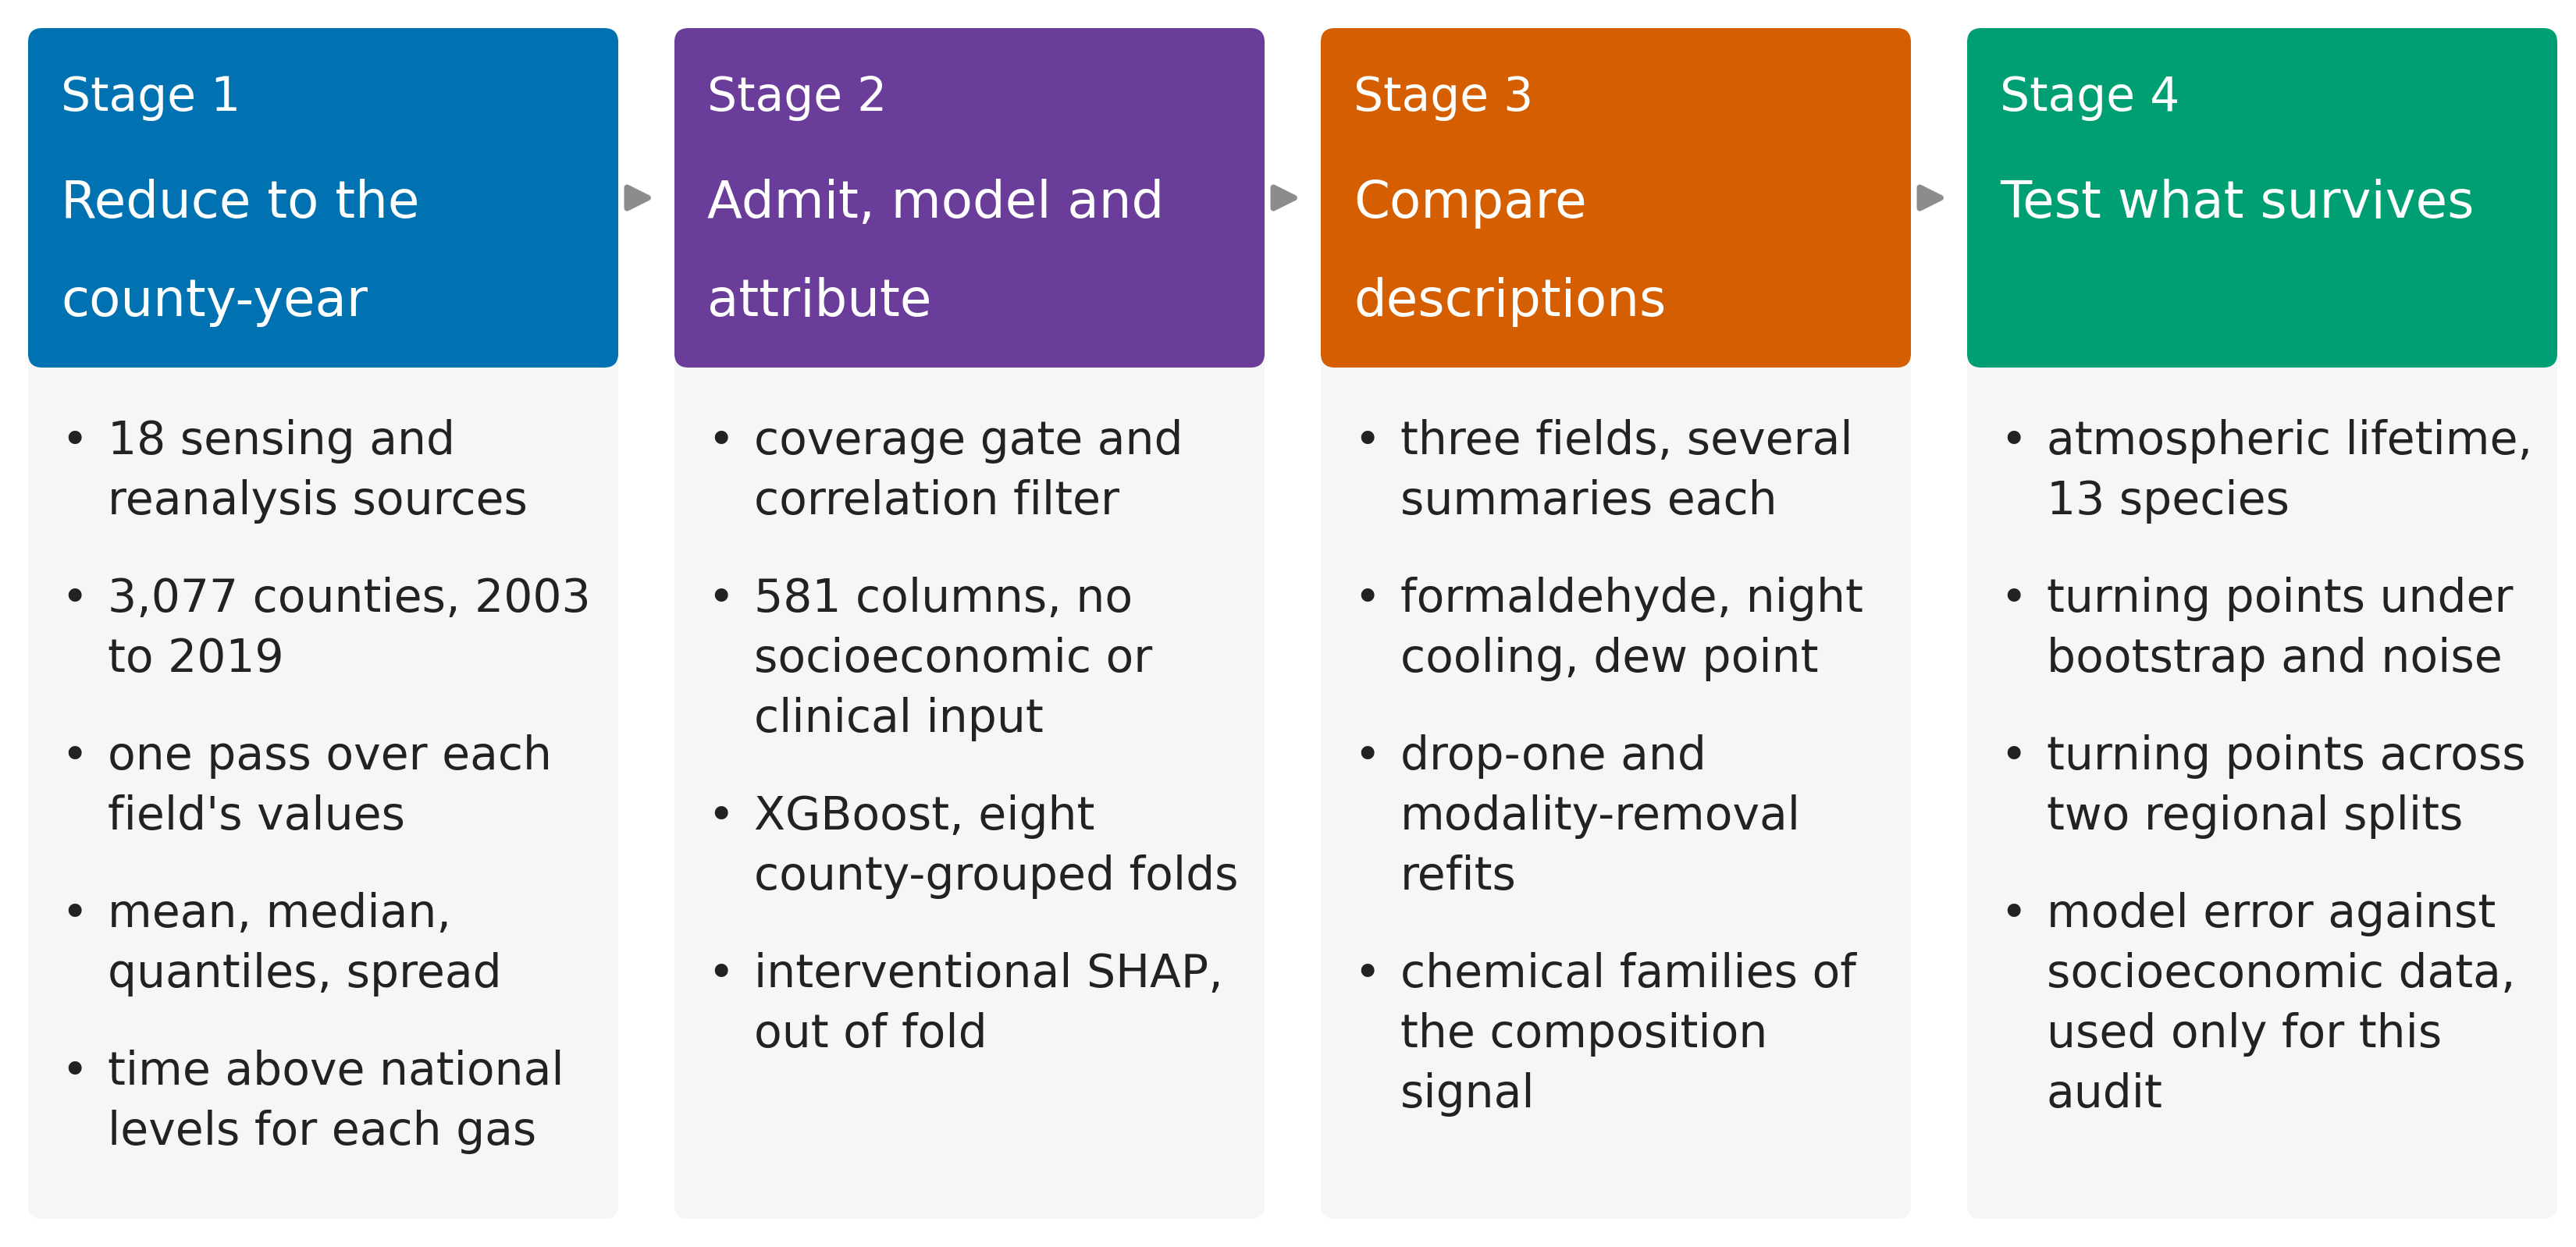
\includegraphics[width=\linewidth]{Figures/Figure01_methodology.png}
\caption{Study design: one set of satellite and gridded fields, each
summarised several ways, feeds one model whose attributions are then tested.
Stage 1 reduces the \Nmodalities{} data sources (the figure calls these sources modalities, and the
block removals modality removals) to the county-year, with several summaries
of each field. Stage 2 admits columns, fits a gradient-boosted model (eXtreme Gradient
Boosting, XGBoost) tested on unseen counties, and attributes its predictions
with SHapley Additive exPlanations (SHAP). Stage 3 compares the summaries of
three fields, refits the model without one or two summaries of a field or
without one block of data, and divides the composition attribution among chemical
families. Stage 4 tests whether the duration advantage varies with atmospheric
lifetime, whether the turning points survive the bootstrap, added noise, and
two regional splits of the country, and whether socioeconomic data predict the
model's error.}
\label{fig:method}
\end{figure}

\subsection{Outcome (Target Variable)}
\label{ssec:m_outcome}
The outcome is county life expectancy at birth for both sexes and all races,
the life-table entry for the age group under one year. Life expectancy at birth
is the average number of years a newborn would live if the death rates at each
age seen in that county and year held for its whole life. The values come from
the small-area estimates of the Institute for Health Metrics and Evaluation
(IHME) for 2000 to 2019~\cite{DwyerLindgren2022}. The estimates borrow
strength across neighbouring counties and adjacent
years~\cite{DwyerLindgren2017}, which raises the skill of the baseline built
from the four nearest counties (Section~\ref{ssec:m_validation}). They also
draw on county
covariates~\cite{DwyerLindgren2017}, so part of the socioeconomic signal in
the error audit (Section~\ref{ssec:m_sdoh}) may enter through the outcome. We
did not carry the published uncertainty of the estimates into the fit.

\subsection{Environmental Data and Reduction to the County-Year}
\label{ssec:m_data}
Table~\ref{tab:data} gives each gridded source with its native resolution, time step, and
number of admitted columns (Section~\ref{ssec:m_model}).

\begin{itemize}[leftmargin=*, topsep=3pt, itemsep=2pt]
\item \textit{Surface temperature and vegetation.} MODIS on the Terra
satellite of the National Aeronautics and Space Administration (NASA) supplies
land-surface temperature (LST), the radiometric skin temperature of soil and
canopy, as 8-day composites at 1\,km~\cite{Wan2014}. Its overpasses are near
10:30 and 22:30 local time, before the early-afternoon
maximum and the pre-dawn minimum of surface temperature. Terra kept its
morning equator crossing until its final inclination manoeuvre in 2020, so the
record used here precedes the orbital drift that
followed~\cite{NASATerra2022}. LST is retrieved only under clear sky, so the
composites favour clear days and nights~\cite{Ermida2019}. MODIS also supplies
vegetation indices. Landsat 5 and 7 supply surface
reflectance and the vegetation indices computed from it, with sensors and sampling that change within the window (Section~\ref{ssec:d_limits}).
\item \textit{Atmospheric composition.} The CAMS global reanalysis of
atmospheric composition (EAC4), produced by the European Centre for
Medium-Range Weather Forecasts (ECMWF), runs atmospheric chemistry inside
ECMWF's weather forecasting model, simulating how gases are emitted, carried,
and transformed. It corrects
the model by assimilating satellite retrievals of four quantities: ozone,
carbon monoxide, nitrogen dioxide, and aerosol optical
depth~\cite{Inness2019}. Its
variables include formaldehyde, nitric oxide, nitrogen dioxide, ozone, carbon
monoxide, sulphur dioxide, nitric acid, the hydroxyl radical, hydrogen
peroxide, peroxyacetyl nitrate, ethane, propane, isoprene, aerosol optical
depth by aerosol type, and modelled particulate matter. Observation constrains
only the assimilated constituents directly; formaldehyde and the other species
are model fields shaped by emission inventories and the model's chemistry.
The biogenic emissions of the reanalysis, the main
summer source of formaldehyde over the United States~\cite{Millet2008}, are
monthly means~\cite{Inness2019}, so the formaldehyde field follows their season
but not their day-to-day changes with weather. Fire emissions, by contrast,
are daily~\cite{Inness2019}. Anthropogenic emissions follow an inventory that ends in 2010 and a scenario afterwards~\cite{Inness2019}, and the bias of surface ozone drifts over time~\cite{Wagner2021} (Section~\ref{ssec:d_limits}). Over the eastern United States
the reanalysis reproduces the level and seasonality of satellite formaldehyde
columns but misses the maxima of individual years~\cite{Wagner2021}.
Ground-level fine particulate matter, particles
with an aerodynamic diameter of 2.5\,micrometres or less (PM$_{2.5}$), comes separately from a product that
combines satellite aerosol optical depth, a chemical transport model, and
ground monitors~\cite{vanDonkelaar2016, Shen2024}. Its panel values
are in units of 10\,\textmu g\,m$^{-3}$, one tenth of the product's native
values, a constant factor that leaves a tree model and every rank-based result
unchanged.

\item \textit{Weather and surface climate.} The fifth-generation ECMWF
reanalysis (ERA5) provides humidity, pressure, wind, snow, terrain height, and
other variables~\cite{Hersbach2020}. TerraClimate supplies monthly water balance,
wind speed, and solar radiation~\cite{Abatzoglou2018}. PRISM supplies daily air temperature, dew
point (the temperature at which air saturates, a measure of its water vapour), vapour-pressure deficit (how far the air is from saturation), and
precipitation~\cite{Daly2008, Daly2015, Daly2021}. Each
4\,km cell was averaged over the year before the county was described by the
distribution of its cells. The minimum dew point of a county is therefore the
annual-mean dew point of its driest cell, not the lowest daily value. It
describes the driest air in the county, which in varied terrain is often on
its highest ground.
\item \textit{Land, soil, and water.} The OpenLandMap soil maps give bulk
density~\cite{Hengl2018}, texture as clay and sand
content~\cite{Hengl2018clay, Hengl2018sand}, acidity~\cite{Hengl2018ph}, and
organic carbon~\cite{Hengl2018oc}. The Global Surface Water record of the Joint Research
Centre (JRC) maps where and how often water is present~\cite{Pekel2016}, and
the Global Human Modification index measures cumulative human pressure on
land~\cite{Kennedy2019}. Night-time lights record the brightness of
settlements, from the Defense Meteorological Satellite Program (DMSP) to 2013
and the Visible Infrared Imaging Radiometer Suite (VIIRS) from
2014~\cite{Elvidge2017}. Each was rescaled within its sensor to the range 0 to
1 (Section~\ref{ssec:d_limits}). A canopy-height model gives the height and cover of
trees~\cite{Tolan2024}. The Cropland Data Layer of the United States
Department of Agriculture (USDA) gives the share of land in each
crop~\cite{Boryan2011}, and the Gridded Livestock of the World the density of
each farm animal~\cite{Gilbert2018}.
\item \textit{Engineered variables.} These combine two or more of the fields
above. Wet-bulb temperature, the lowest temperature to which evaporation can
cool a wet surface, was computed with the empirical formula of Stull, which
assumes sea-level pressure and errs by up to 1\,\textdegree C~\cite{Stull2011}.
At the lower pressure of high ground it therefore overstates the wet-bulb
temperature. Its night-time form combines the county's annual-mean daily
minimum temperature with the annual-mean dew point of its driest cell. It is
therefore an index of night-time moisture stress, not the wet-bulb temperature
of any one place or night. Its warm-hour form combines the county's annual-mean
daily maximum temperature with its annual-mean dew point. The others are the
heat index and related heat-stress
indices, dew-point depression, night cooling efficiency
(Section~\ref{ssec:m_descriptions}), and ratios of atmospheric species, such as
formaldehyde to nitrogen dioxide.
\end{itemize}

% tables_data.tex -- written by analysis/build_paper_constants.py
% Column counts are read from the model's ranking; do not edit by hand.
\begin{table}[H]
\caption{Data sources and the outcome, with each product's native resolution and the number of its columns among the 581 the model sees. Single maps enter every year with the same value. The three Sentinel missions were acquired but none of their columns met the coverage gate.\label{tab:data}}
\centering\footnotesize
\setlength{\tabcolsep}{4pt}
\begin{tabular}{@{}>{\raggedright\arraybackslash}p{3.0cm}>{\raggedright\arraybackslash}p{3.7cm}>{\raggedright\arraybackslash}p{1.8cm}>{\raggedright\arraybackslash}p{1.8cm}r@{}}
\toprule
Source & Variables, for example & Spatial resolution & Time step & Columns \\
\midrule
MODIS land-surface temperature (Terra) & Day and night land-surface temperature & 1 km & 8-day & 11 \\
MODIS vegetation indices & Normalised difference and enhanced vegetation indices & 500 m & 16-day & 10 \\
Landsat 5 and 7 & Surface reflectance, vegetation indices & 30 m & 16-day revisit & 72 \\
Sentinel-1 & Radar backscatter & 10 m & 6 to 12 days, from 2014 & 0 \\
Sentinel-2 & Optical reflectance & 10 to 60 m & 5 days, from 2015 & 0 \\
Sentinel-5P & Trace gases, aerosol index & About 5 km & Daily, from 2018 & 0 \\
Satellite fine particulate matter & Ground-level PM$_{2.5}$ & About 1 km & Annual & 7 \\
Night-time lights (DMSP, VIIRS) & Settlement brightness, rescaled within each sensor & About 1 km; 500 m & Annual & 7 \\
Global Surface Water (JRC) & Water occurrence and class & 30 m & Annual & 6 \\
Global Human Modification & Human pressure on land & 1 km & Single map & 5 \\
Canopy height & Canopy height and cover & 1 m & Single map & 16 \\
Cropland Data Layer (USDA) & Share of land in each crop & 30 m & Annual & 105 \\
CAMS global reanalysis (EAC4) & Trace gases, aerosol optical depth, particulate matter & 0.75\textdegree{} (about 80 km) & 3-hourly & 67 \\
ERA5 reanalysis & Humidity, pressure, wind, snow, terrain height & 0.25\textdegree{} (about 28 km) & Hourly & 18 \\
PRISM & Air temperature, dew point, vapour-pressure deficit, precipitation & 4 km & Daily & 80 \\
TerraClimate & Water balance, wind, solar radiation & About 4 km & Monthly & 40 \\
OpenLandMap soil maps & Bulk density, texture, acidity, organic carbon & 250 m & Single map & 58 \\
Gridded Livestock of the World & Density of each farm animal & About 10 km & Reference years, linear between & 28 \\
Engineered from the above & Wet-bulb and heat indices, night cooling efficiency, species ratios & Of the inputs & Annual & 51 \\
\midrule
IHME small-area estimates & Life expectancy at birth, both sexes, all races (the outcome) & County & Annual & -- \\
\bottomrule
\end{tabular}
\end{table}




We reduced the satellite fields to county polygons with the Google Earth Engine
platform~\cite{Gorelick2017}. The CAMS and ERA5
fields come from the county extraction of the earlier studies of these
fields~\cite{Ruwali2026multi, Shrestha2026exp}. Those studies downloaded them
from the Copernicus data stores on their native grids and time steps,
interpolated each time step multilinearly to points along the county boundary,
and averaged over those points, not over the county's area (Section~\ref{ssec:d_limits}).
The county is
coarser than most inputs, though finer than the CAMS grid. In
the Albers equal-area projection, the median county covers the area of a
\CountyScaleMed{}\,km square, and the middle 80\% lie between
\CountyScaleLo{} and \CountyScaleHi{}\,km. Products finer than 250\,m were
therefore reduced at a scale coarser than their own: the 30\,m products at
250\,m and canopy height at 10\,m. The others were reduced at or near their own
resolution.
Predictors for year $t$ were matched to the outcome for year $t$
(Section~\ref{ssec:d_limits}). Soils, canopy
height, and human modification are single maps and entered every year with the
same value; livestock density changes linearly between its reference years and
is constant before 2010.

The reduction also returned several summaries of the same values. For
gridded fields other than CAMS and ERA5 they were taken over the cells of the
county: the mean, median, minimum, maximum, a set of percentiles, and the
standard deviation. For the CAMS and ERA5 fields the summaries were taken over the
year's time steps, and for the atmospheric species they included the share of
time above national reference levels. We call each such statistic of a field
a summary of it. Two summaries of a field therefore differ
in the statistic but not in the measurement.
\subsection{Several Summaries of One Field}
\label{ssec:m_descriptions}
We compared summaries in three fields: formaldehyde from the CAMS reanalysis,
night cooling from MODIS LST, and dew point from the station-based PRISM
climate grid. We chose them after seeing the production ranking
(Section~\ref{ssec:m_attribution}): each has a leading summary among its top
eleven variables and an
admitted mean form (Section~\ref{ssec:m_model}). Section~\ref{ssec:r_two} sets
these three against the ratio of the most to the least attributed summary in
each field summarised over county cells with more than one admitted summary.

\textit{Concentration and duration.} For an atmospheric species $c$ in county $i$ and year $t$, with values
$x_{c,i,t}(s)$ at the $S_t$ three-hourly time steps of the year (about 2,920), concentration
is the annual mean. Duration is the share of the year, in per cent, spent
above a national reference level~\cite{Shrestha2026exp},
\begin{equation}
D^{(K)}_{c,i,t}
= \frac{100}{S_t}\sum_{s=1}^{S_t}\mathbf{1}\!\left[x_{c,i,t}(s) > q_{c,t}^{(K)}\right],
\label{eq:duration}
\end{equation}
where $q_{c,t}^{(K)}$ is the $K$th percentile, across all counties (test counties
included, Section~\ref{ssec:m_model}), of the
annual mean of species $c$ in year $t$. The indicator $\mathbf{1}[\cdot]$
equals one when its condition holds.

Because the reference is one national number in each year, a given value of $D$
means the same share of time above the same ambient level in every county of
that year. $D$ does not record how far above the reference a county goes, and
it describes an ambient field, not what people breathe. We computed it at $K = 75$ and $K = 90$, so each species was offered to the model as
its concentration and two durations.

\textit{Two constructions of night cooling.} Night cooling efficiency (NCE)
is the day-to-night drop in LST divided by the daytime
value, both in degrees Celsius. Because the Celsius zero is arbitrary, NCE
rises as the daytime temperature falls even when the drop is unchanged: a
12\,\textdegree C drop gives 0.40 at 30\,\textdegree C and 0.60 at
20\,\textdegree C. Two
engineered layers built it from the same MODIS product with different summary
statistics,
\begin{equation}
\text{NCE}_{\text{tail}} = \frac{\text{LST}^{\text{day}}_{\text{p90}}
  - \text{LST}^{\text{night}}_{\text{p10}}}{\text{LST}^{\text{day}}_{\text{p90}}},
\qquad
\text{NCE}_{\text{mean}} = \frac{\text{LST}^{\text{day}}_{\mu}
  - \text{LST}^{\text{night}}_{\mu}}{\text{LST}^{\text{day}}_{\mu}},
\label{eq:nce}
\end{equation}
where p90 and p10 are the 90th and 10th percentiles of the county's
pixels and $\mu$ is their mean. The tail form is the NCE of the earlier
nocturnal study~\cite{Ahmad2026night}. Because its warmest daytime and coolest
night-time pixels need not lie in the same places, it also records contrasts in
land cover within the county. Recomputation confirmed both formulas:
among all ordered pairs of the \NCEcandCols{} temperature columns from
\NCEcandSrc{} instruments under five ratio forms, exactly one reproduced each
layer (maximum absolute difference \NCEmaxdiffMean{} for the mean form). The
two layers correlated at \NCEcorr{}.

\textit{Seven summaries of dew point.} All seven summaries of the PRISM dew
point passed admission: the mean, median, minimum (the driest cell),
maximum, 10th and 90th percentiles, and standard deviation (its
variability).

Column names give the field and, where present, the statistic. Grouped by
field, the columns summarised over the cells of each county give
\StatFieldsTotal{} fields with more than one admitted summary. The CAMS and
ERA5 fields and the engineered
layers, including both constructions of NCE, are not among them. Nor are the
MODIS vegetation indices, whose column names end in a scaling tag rather than
a statistic.

\subsection{Admission, Model, and Cross-Validation}
\label{ssec:m_model}
The reduction produced \CatCandidates{} candidate columns. A coverage gate kept
a column only if it was present in at least
\CoverageThreshold{}\% of the county-years of the whole window and took at
least three distinct values. The gate stopped a product available only
in later years from letting the model learn the year in place of the place.
The gate also dropped any column derived from the outcome or from socioeconomic
or clinical sources; \CatAdmitted{} columns passed. A
second pass, the correlation filter, removed near-constant columns and one
member of any pair whose
absolute Pearson correlation reached \CollinearCut{}, a cut that removed only
near-duplicates, leaving the \Nfeatpruned{} columns the model saw. These
admitted columns are the model's variables. Neither pass used the values of the
outcome.

A declared list of physiologically motivated patterns was protected. It covered
heat indices, wet-bulb temperature, and wind chill; dew point and humidity,
including total column water vapour; minimum temperature, night-time LST, and
the diurnal temperature range; and night cooling. It also covered
vapour-pressure deficit, counts of hot nights and days, and formaldehyde,
nitrogen dioxide, ozone, and PM$_{2.5}$. The correlation filter never dropped a
protected column, so the two durations of formaldehyde, which correlated at
\HchoDurCorr{}, survived together; both constructions of NCE and the
minimum dew point were also protected. Of two unprotected columns it dropped the later one in the
data table, and of a mixed pair the unprotected one.

The model is a gradient-boosted tree ensemble~\cite{Friedman2001}:
\RefitTrees{} decision trees, each correcting the errors of those before it.
Trees accept correlated
inputs on different scales without transformation, and their SHAP values can be
computed exactly~\cite{Lundberg2020}. We fitted the model with
eXtreme Gradient Boosting (XGBoost)~\cite{Chen2016}, chosen over Categorical
Boosting (CatBoost)~\cite{Prokhorenkova2018} on identical splits. Both learners
used settings fixed in the pipeline before the model was fitted and not tuned
on these data (Appendix~\ref{app:learner}).

Cross-validation used eight county-grouped folds, each tested by a model trained on the other
seven, so no county appeared
in both training and test~\cite{Roberts2017}. Every reported skill is out of
fold and, except in the two temporal checks of Section~\ref{ssec:m_validation},
measured on test counties. We call the model fitted under these
eight folds the production model. Skill is the coefficient of
determination ($R^{2}$), one minus the ratio of the mean squared prediction error to the variance of life expectancy across
county-years, together with the mean absolute
error, the average size of a miss in years. $R^{2}$ falls below zero when the predictions do worse than the mean. The $R^{2}$ interval bootstrapped
county-years with predictions held fixed; it is likely too narrow, because a county's years were resampled as independent. The residual of a county-year is
observed minus predicted life expectancy.

\subsection{Baselines and Tests of Skill}
\label{ssec:m_validation}
We fitted five baselines: the training mean; the
training mean by year; night-time lights alone; latitude, longitude, and year;
and the same year's life expectancy of the four nearest training counties,
weighted by inverse distance. That last baseline used
information the model was never given. We also fitted the model under folds
grouped by state, so that most of a county's neighbours are held out with it;
the baselines kept the county-grouped folds.

We measured data sufficiency by a learning curve on growing shares of counties
under four folds. We also measured the mean absolute error within five brackets of
observed life expectancy, each including its lower bound (60--70, 70--74, 74--76.5, 76.5--79, and 79--95 years). To find whether skill comes from differences between
counties or from change within a county, we permuted the outcome across all
rows, within each county, and between whole counties.
Leave-one-year-out and forward-chaining folds (training on earlier years, testing on later ones) measured temporal behaviour.

We also removed each of the \LOOnModalities{} feature blocks in turn and
refitted the model. The blocks are the
sources of Table~\ref{tab:data} that have admitted columns and the two groups
of engineered variables. The loss of skill measures what a kind of data adds
that the others cannot replace.

The production model and the block removals were fitted on the Juno cluster of the
University of Texas at Dallas in Python 3.10.12. The baselines and the drop-one refits
(Section~\ref{ssec:m_refit}) ran in Python \VerPython{} with XGBoost
\VerXgb{}, SHAP \VerShap{}, and scikit-learn \VerSklearn{} and shared a second
set of folds. Every script is seeded, and the folds of the second set are stored with
the code, because scikit-learn does not assign equal-sized groups to the same
folds in every version.

\subsection{Attribution}
\label{ssec:m_attribution}
The main attribution is SHAP in its
interventional tree form, TreeSHAP~\cite{Lundberg2017, Lundberg2020,
Janzing2020}. A SHAP value divides one prediction among the inputs by
averaging, over all orders in which the inputs could be added, the change each
input makes when added~\cite{Shapley1953}. The interventional form fills an absent input from a
background sample independently of the inputs present. Under the conditional form, an input that
merely restates another can receive attribution for it, because
conditioning on the first also moves the second~\cite{Janzing2020}. For near-duplicate
columns, the interventional form also evaluates the model at combinations of
values that never occur together, so the split of attribution between them partly
rests on points outside the data~\cite{Kumar2020, Hooker2021}. The refits of Section~\ref{ssec:m_refit}
test that split.

We computed the
production ranking out of fold: in each of the eight folds, the fold's model
attributed 4,000 county-years of its test counties against a background of
1,000 county-years drawn from its training counties. A column's importance is
its mean absolute SHAP value, in years of life expectancy, averaged over the
folds, and its rank is its place among the \Nfeatpruned{} variables. A county
bootstrap and new seeds tested the stability of this ranking. We refitted without the
\InflDropN{} counties with the largest mean absolute out-of-fold residual. We
attributed that refit by path-dependent TreeSHAP, which needs no background
sample~\cite{Lundberg2020}, and counted the production top \InflTopK{} variables still in
its top \InflTopK{}.



\subsection{Drop-One Refits}
\label{ssec:m_refit}
A refit experiment, in the manner of leave-one-covariate-out
importance~\cite{Lei2018}, tested whether a large attribution gap between two
correlated columns comes from the way attribution is split inside one fitted model
or from a difference in what the columns carry. It removed one construction of
NCE at a time, first the tail form and then the mean form, and refitted on the
second set of \RefitFolds{} folds (Section~\ref{ssec:m_validation}). It measured
the refitted model's out-of-fold skill, which
involves no attribution, and the attribution of the construction left behind.
If the two were one variable measured twice, skill would hold and the removed
construction's attribution would pass to the one left behind. If either
carried information that no other column holds, skill would fall. If other
columns also carried the removed construction's information, skill would hold but little attribution
would pass to the one left behind. The same design removed the two
formaldehyde durations, singly and together. These refits used the production
settings of the learner (\RefitTrees{} trees, learning rate \RefitLR{}, maximum
depth \RefitDepth{}; Table~\ref{tab:learner}). Each NCE refit was attributed on
\RefitShapN{} county-years against a background of \RefitShapBg{}, and each
formaldehyde refit on \HchoDropShapN{} against \HchoDropShapBg{}. Skill was
compared only among refits on these folds, against a refit with all
\ArmAllN{} columns (Section~\ref{ssec:r_model}).

\subsection{Atmospheric Composition and Lifetime}
\label{ssec:m_lifetime}
We divided the composition attribution among chemical families and tested
whether the duration advantage varies with atmospheric lifetime. Throughout this paper, the lifetime of a species is its
atmospheric lifetime $\tau$: the tropospheric burden of the species divided by
its total removal rate~\cite{Seinfeld2016}. The chemistry scheme of the CAMS forecasting system
uses the same definition for its own budgets~\cite{Flemming2015}.
If the sources of a species stopped, its amount would fall to $1/e$, about
37\%, of its starting value after $\tau$; this e-folding time is longer than
the half-life, $\tau \ln 2$.

We assigned each of the \CompN{}
admitted composition columns by its name to one of \FamN{} chemical families
and computed each family's share of the summed attribution of all composition
columns. The families include the oxygenated species (formaldehyde and
hydrogen peroxide), alkanes, sulphur species, reactive nitrogen, oxidants, and
particulate matter. For every species with both durations admitted, we
divided the importance of the time above the 75th percentile by that of the time above the 90th.
We then paired every
species' duration and concentration columns, \LtPairs{} pairs over
\LtSpecies{} species (Table~\ref{tab:species}), took the ratio of the duration column's
importance to the concentration column's (the duration advantage), and tested whether the per-species median ratio falls as
lifetime rises. Lifetimes, which the reanalysis does not output, came from the
literature~\cite{Seinfeld2016,
AtkinsonArey2003, FinlaysonPitts2000, Lelieveld2016, Textor2006, Young2013,
Fischer2014}. The test was a one-sided permutation test of Spearman's
correlation over \LtPerms{} permutations, by species, since one species' pairs are not independent. A one-sided
Mann--Whitney test at the 5\% level, again by species, compared the ratios of
short-lived and longer-lived species at a boundary of \LtCutoff{} days fixed in
advance and at all \LtSweepN{} boundaries, uncorrected for multiplicity. We also
multiplied each lifetime by ten raised to an independent uniform draw between
$-$\LtValueDex{} and \LtValueDex{}, \LtValueDraws{} times, counted the draws in which the
correlation stayed negative, and left each species out in turn.

\subsection{Turning Points and Their Stability Criterion}
\label{ssec:m_turning}
A turning point is the value of a variable at which its attribution changes sign. We located it on the attribution curve, the plot of a
variable's SHAP value against its own value, using \GateShapN{} county-years
attributed by the model fitted to all counties against a background of
\InvShapBackground{}. The observations were placed in 45 equal-count bins
between the 1st and 99th percentiles, so that each median rests on several
hundred county-years. The located value is where a smoothing spline
through the bin medians crosses zero (the steepest crossing where there are
several).

SHAP values are centred at the model's mean prediction over the
background sample, so a zero-crossing marks a change from raising the prediction above that level
to lowering it, or the reverse, not by itself a transition from a
protective to a harmful exposure. Under the interventional form, a variable's
attributions average to zero over the background sample, so the crossing of a
monotone curve falls near the middle of its distribution. The curve of a
variable with a near-collinear partner, such as the minimum dew point, rests
partly on the never-observed combinations of values described in
Section~\ref{ssec:m_attribution}; accumulated local effects avoid
them~\cite{Apley2020}. For each turning point we interpret, we report the
share of county-years above it.

Because any estimator returns a number for any curve, including a flat one,
we fixed the criterion for accepting a located value before seeing any
estimate. We drew \TpBoot{} bootstrap resamples of the attributed county-years
with replacement, treating a county's years as independent, reusing one background sample, and not refitting the model, so the intervals are likely too narrow (Section~\ref{ssec:d_turning}) and are
conditional on that model. A candidate is stable only if three conditions
hold. A crossing
must usually exist: it is found in at least 60\% of resamples. It must be
precisely located: the interval between the 2.5th and 97.5th percentiles of the
located values is narrower than 40\% of the variable's range between its 1st
and 99th percentiles. The
full-sample value must agree with the resamples by lying inside that interval.

The criterion was applied to \TpTotal{} candidates
(Table~\ref{tab:turning}). Three of them, hereafter the three moisture
and night-cooling variables, are the minimum dew point, the night-time
wet-bulb temperature, and the tail form of NCE. Two describe composition: the
formaldehyde duration and the ratio of formaldehyde to nitrogen dioxide, which
indicates whether nitrogen oxides or volatile organic compounds limit ozone
formation~\cite{Duncan2010}. Two are alternative forms: the mean form of NCE
and the warm-hour wet-bulb temperature. Two describe temperature: mean
night-time LST and the minimum (coldest-cell) temperature, the annual-mean
daily minimum of that cell. The other two are the share of cropland in corn and the annual
mean of satellite-derived PM$_{2.5}$.

Against a null, we permuted each
candidate's attribution against its own predictor \NullCrossDraws{} times and
reran the whole procedure with \NullCrossBoot{} bootstrap resamples per draw.
We also shifted each curve upward until it no longer crossed zero, where the
procedure should find nothing. Against random error in the predictors, we added Gaussian noise of 1,
2, 5, and 10\% of each predictor's standard deviation, \PertDraws{} times at
each level, and relocated the crossing. We expressed each shift in widths of
the reported interval. Against climate, we cut the panel into western and
eastern halves by county centroid (\RegMerMatched{} of the \GateShapN{} attributed
county-years had a matched centroid) and relocated each crossing within each half. The shift is the absolute west-minus-east difference, in the variable's units and as a share of its 1st-to-99th-percentile range. We cut at the
100th meridian, the conventional boundary between the semi-arid western Great
Plains and the humid east~\cite{Seager2018}, and at the median longitude
(\RegMedCut{}\,\textdegree W). Both halves come from one attributed
sample of one model, so the split tests the fitted model, not physiology.

The raw minimum dew point and minimum
temperature are nearly collinear, so we correlated their attributions (Pearson) to check
that a turning point in one is not a copy of one in the other. We
relocated the dew-point crossing within each quartile of the minimum
temperature to see where in the temperature range it holds.

\subsection{Model Error and Socioeconomic Conditions}
\label{ssec:m_sdoh}
The error audit tested the model's residuals against the social determinants of health, the
conditions in which people are born, live, work, and age~\cite{Marmot2008}. The socioeconomic data
come from the Social Determinants of Health database of the Agency for
Healthcare Research and Quality (\ResSdohYearLo{} to \ResSdohYearHi{}). We kept the \ResSdohN{}
columns with a value in at least 80\% of counties and more than five distinct
values, and averaged each over the years of each county. Of these, \ResAcsN{}
come from the American Community Survey of the United States Census Bureau;
the rest come from the County Health Rankings~\cite{Remington2015}, the Small
Area Income and Poverty Estimates, and county economic series.

We averaged the out-of-fold residual within each county over \YearStart{} to
\YearEnd{}, a longer window than the socioeconomic averages, and measured its
spatial structure by Moran's $I$~\cite{Moran1950}, tested against
\MoranPerm{} permutations. Here Moran's $I$ is the slope of the mean residual
of a county's four nearest neighbours on its own residual (row-standardised
weights). We counted the counties overpredicted by \ResMissYears{} years or more. We then predicted the county residual under eight folds grouped by
state, once from the \ResSdohN{} socioeconomic columns and once from the
\ResEnvN{} environmental columns the model had used. The learner was histogram
gradient boosting, which accepts missing values. Because some County Health
Rankings columns describe health behaviour and status (smoking, obesity, and
physical inactivity), we repeated the audit without the Rankings (\ResNoChrN{} remained)
and with the American Community Survey columns alone. We correlated six
indicators named in advance (poverty, median household income, unemployment,
uninsurance, bachelor's degree attainment, and disability) with the residual
by Spearman's rank correlation, which assumes no linear form. The Holm
procedure~\cite{Holm1979} corrected for testing six at once; counties were treated
as independent, so the $p$-values are too small.


%% ======================================================================
\section{Results}
\label{sec:results}

\subsection{Predictive Skill}
\label{ssec:r_model}
From satellite and gridded data alone, the model predicted the life expectancy of \Ncounties{} counties from \YearStart{} to \YearEnd{}
(\Nobs{} county-years; Figure~\ref{fig:performance}A) with out-of-fold $R^{2}$ = \Rtwo{} under eight county-grouped folds (Section~\ref{ssec:m_model}). The 95\%
interval was \RtwoCIlo{} to \RtwoCIhi{}, likely too narrow, and the mean absolute error \MAEmodel{} years.
On the second set of folds, which the baselines share, the model reached
\ArmAllRtwo{} and scored above every baseline (Section~\ref{ssec:m_validation}), including the four nearest counties'
life expectancy (\BlKnn{}; the gap has no paired test). Holding out whole states lowered skill to
\HoldStateRtwo{}, the figure for prediction in a region the model
has not visited. CatBoost reached \CatBoostRtwo{} out of fold, so the choice of learner
moved skill by less than one hundredth.

Skill has nearly levelled off with the number of counties seen: under four
folds, it was \LcTenRtwo{} with a tenth of them, \LcHalfRtwo{} with half, and
\LcFullRtwo{} with all (Figure~\ref{fig:performance}B). Out-of-fold error was largest at
the extremes of observed life expectancy, chiefly in its lowest bracket: the
mean absolute error was \BrLowMAE{} years there against \BrMidMAE{} in the
bracket holding the most county-years (Figure~\ref{fig:performance}C).

Shuffling years within each county left out-of-fold skill at \NullSkillWithin{}, whereas
swapping whole series between counties removed it (\NullSkillBetween{};
Figure~\ref{fig:performance}D): the model explained differences between
counties, not one county's path through time. Leaving one year out ($R^{2}$ =
\LoyoMean{}) and forward chaining (\FwdMean{}) keep every county in training,
so they measure persistence, not skill on new counties.

Of the \LOOnModalities{} feature blocks, removing soil properties or
night-time lights raised out-of-fold skill on the production folds. Removing the \LOOcamsN{}
atmospheric composition columns gave the largest loss, changing $R^{2}$ by \LOOcams{}; no block has a reported uncertainty.

\begin{figure}[H]
\centering
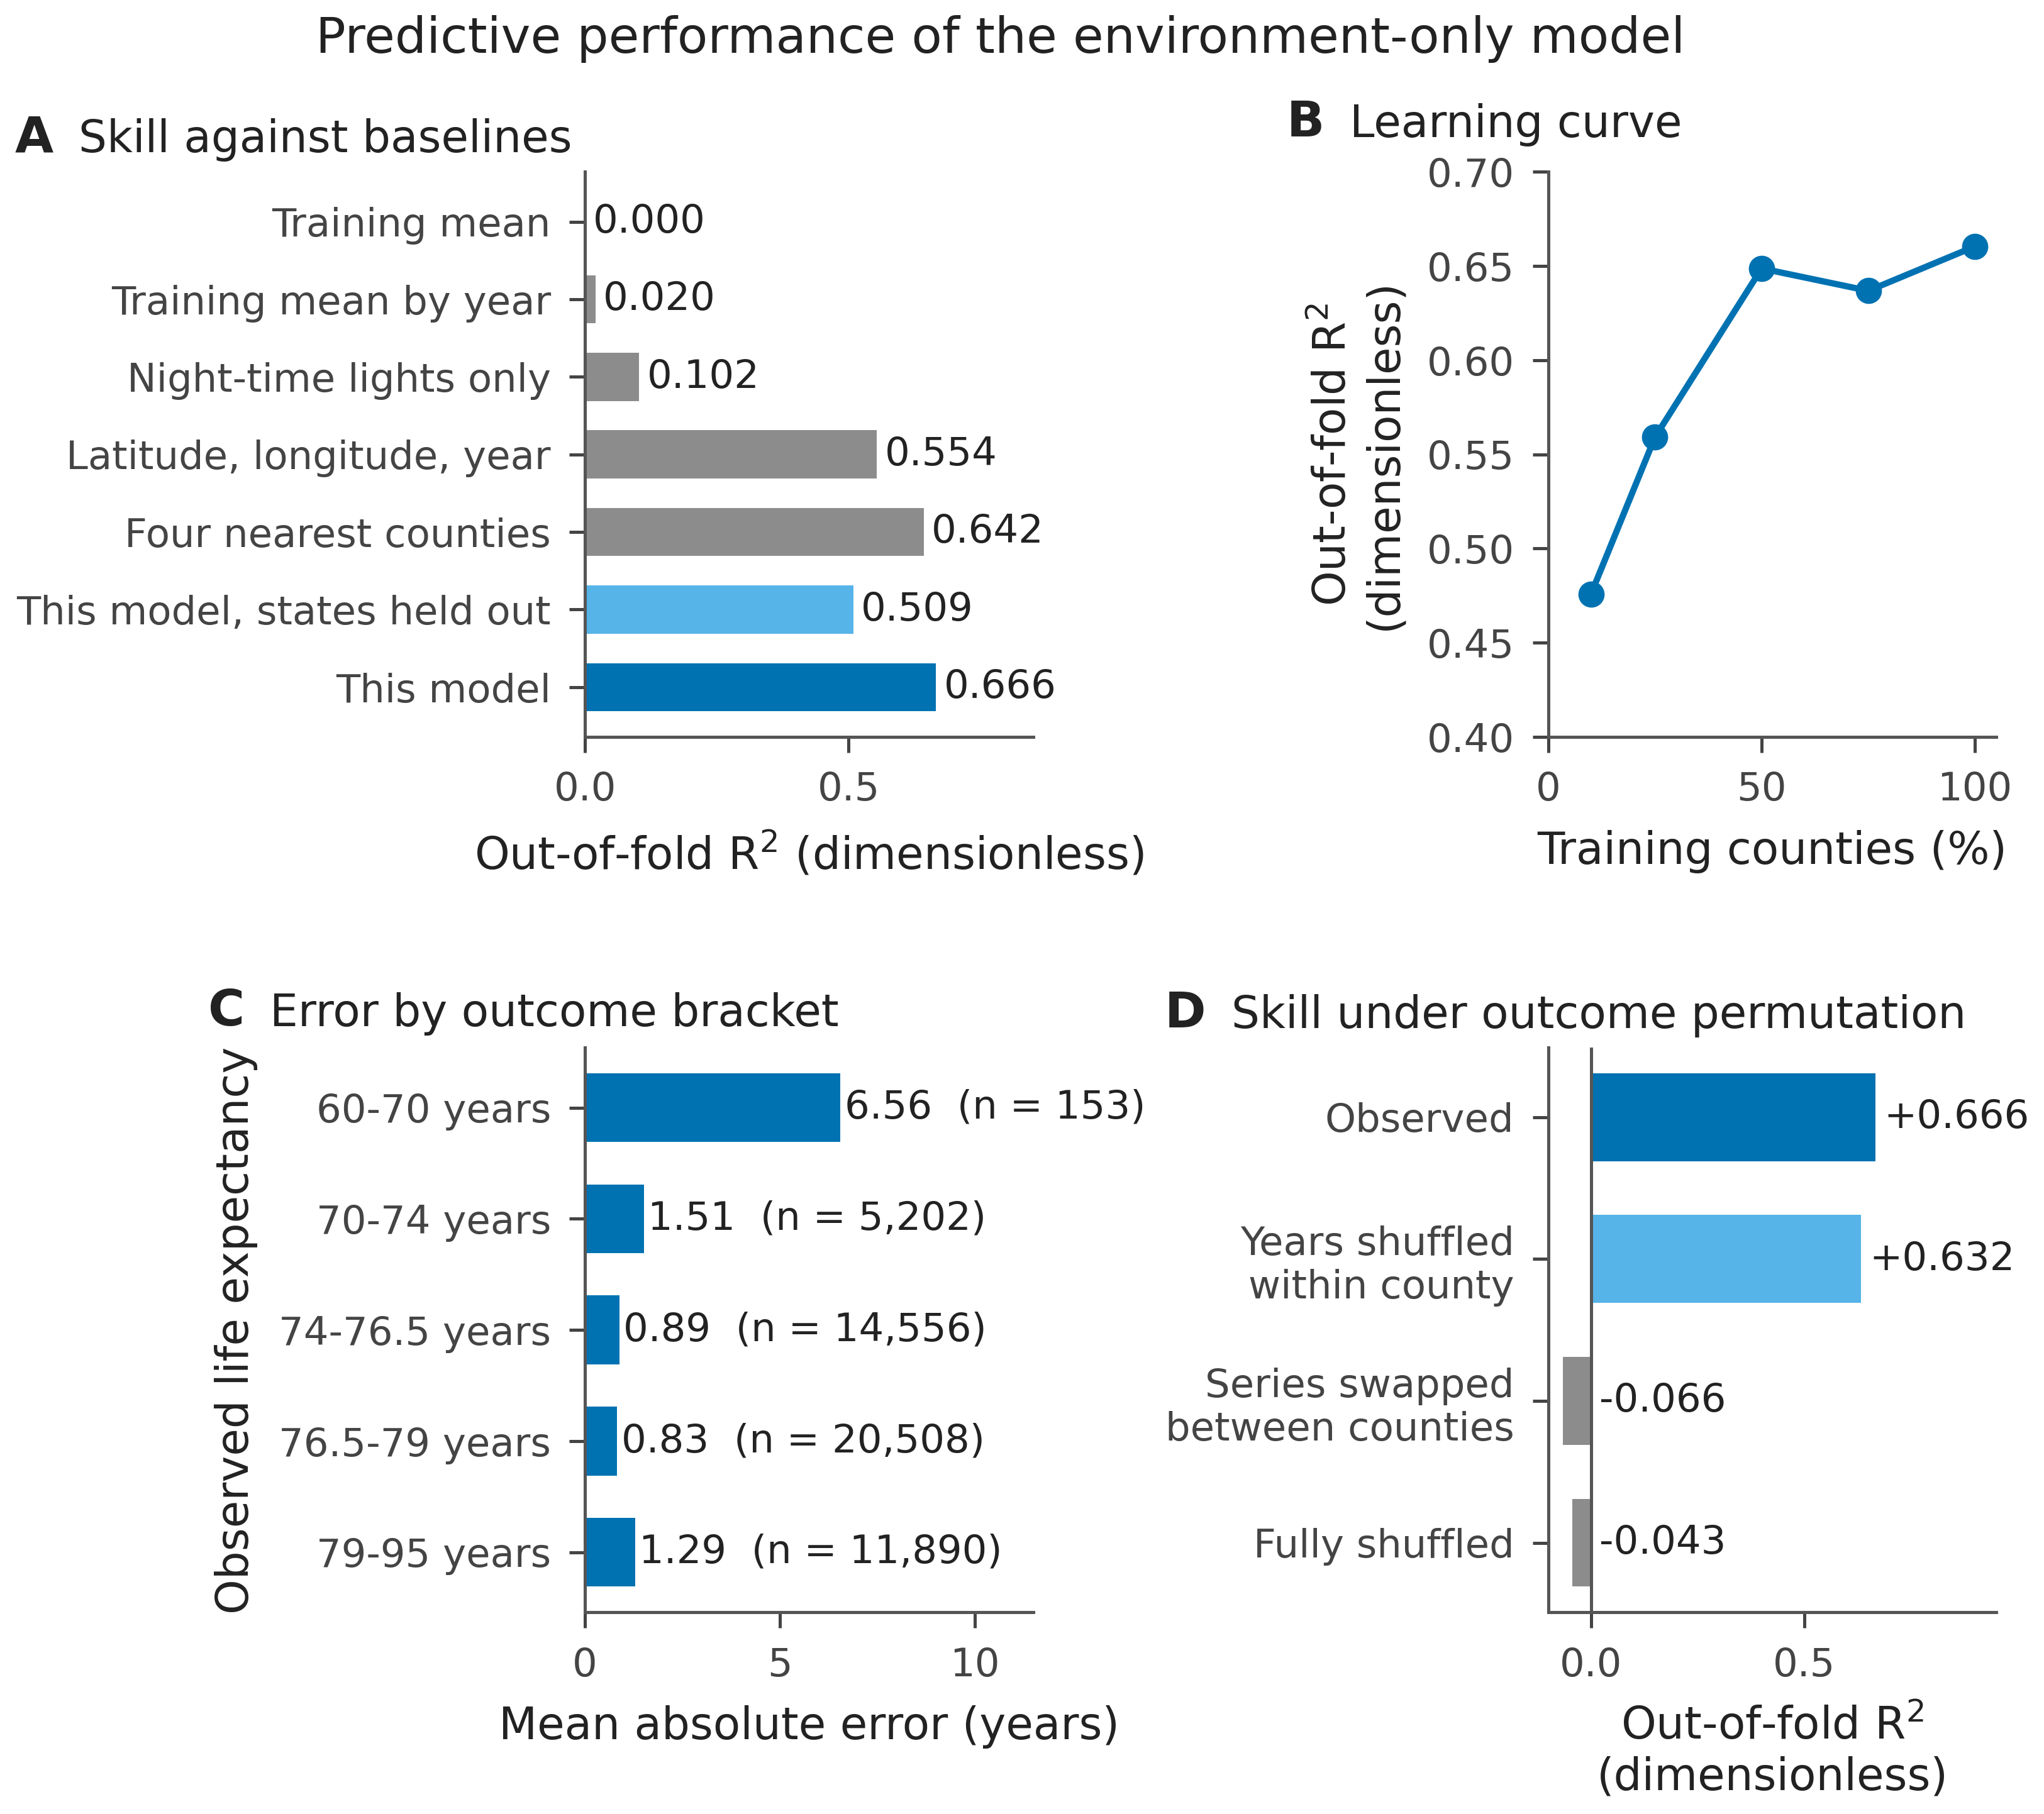
\includegraphics[width=\linewidth]{Figures/Figure02_performance.png}
\caption{From satellite and gridded data alone, the model predicts life
expectancy in unseen counties with a higher $R^{2}$ than every baseline, including the life
expectancy of the four nearest counties. (A) Out-of-fold
coefficient of determination ($R^{2}$) of the model (dark blue), of the model
with whole states held out (light blue), and of five baselines (grey). The
baselines were fitted under county-grouped folds only, on a second fold set on
which the model reaches \ArmAllRtwo{} (Section~\ref{ssec:r_model}). (B) Learning curve over the share of counties
used for training, under four county-grouped folds, so its full-data value
(\LcFullRtwo{}) sits below the eight-fold \Rtwo{} of panel A. (C) Out-of-fold mean absolute error (years) by observed life-expectancy bracket, with
the number of county-years ($n$). (D) $R^{2}$ on the observed outcome (dark
blue) and on three scrambled versions (light blue and grey).}
\label{fig:performance}
\end{figure}

\subsection{Effect of the Summary Statistic on Attribution}
\label{ssec:r_two}
On the first question, with the data held fixed, the model's most and least attributed summaries of a
field differed by a median factor of \CensusMedianSpread{}. The
\StatFieldsTotal{} fields are those summarised over county cells with several admitted
summaries; formaldehyde and NCE are not among them
(Section~\ref{ssec:m_descriptions}). The leading variable
was the share of the year a county's formaldehyde spent above the 75th
percentile of that year's county annual means, with a mean absolute
attribution (Section~\ref{ssec:m_attribution}) of \HchoDurSHAP{} years. The annual mean of the same field from the same product
ranked \HchoConRank{}th of \Nfeatpruned{} variables, at \HchoConSHAP{} years; no rank here carries an interval.
The leader carried \HchoRatio{} times as much (Figure~\ref{fig:three}A), perhaps partly because the yearly reference level of Equation~(\ref{eq:duration}) removes a uniform national trend from the duration but not from the mean. CAMS grid cells are wider than most counties (Section~\ref{ssec:m_data}), so the leader's attribution may partly reflect regional position. The
two constructions of NCE,
built from one MODIS product and correlated at \NCEcorr{}, ranked
\NCEpctRank{}nd and \NCEmeanRank{}rd, a factor of \NCEratio{} apart
(Figure~\ref{fig:three}B). Of the \DPSummariesN{} summaries of the PRISM dew
point, the minimum ranked \DPMinRank{}th, with \DPProfileRatio{} times the
attribution of the next-best summary, the standard deviation (rank
\DPNextRank{}); the mean ranked \DPMeanRank{}st (Figure~\ref{fig:three}C). Extremes,
percentiles, and the standard deviation taken over a county's cells depend on
how many cells it has and the relief they span, so these summaries can also
carry county size and terrain. In the full ranking, each leading
summary sat near the head and each mean form in the long tail
(Figure~\ref{fig:three}D). These three fields were chosen after seeing the ranking
(Section~\ref{ssec:m_descriptions}), so they show how strongly the summary
can change attribution, not how strongly it usually does. Not every mean sat in the tail: for soil bulk
density, the 90th percentile and the mean
ranked \SoilPninetyRank{}th and \SoilMeanRank{}th, a factor of \SoilRatio{}
between them.

As a check on the ranking, a refit without the \InflDropN{} worst-predicted
counties kept \InflOverlap{} of the top \InflTopK{} variables under
path-dependent TreeSHAP (Section~\ref{ssec:m_attribution}), with the tail form of NCE first. Its $R^{2}$ on the
rest, \InflDropRtwo{}, is higher by construction.

\begin{figure}[H]
\centering
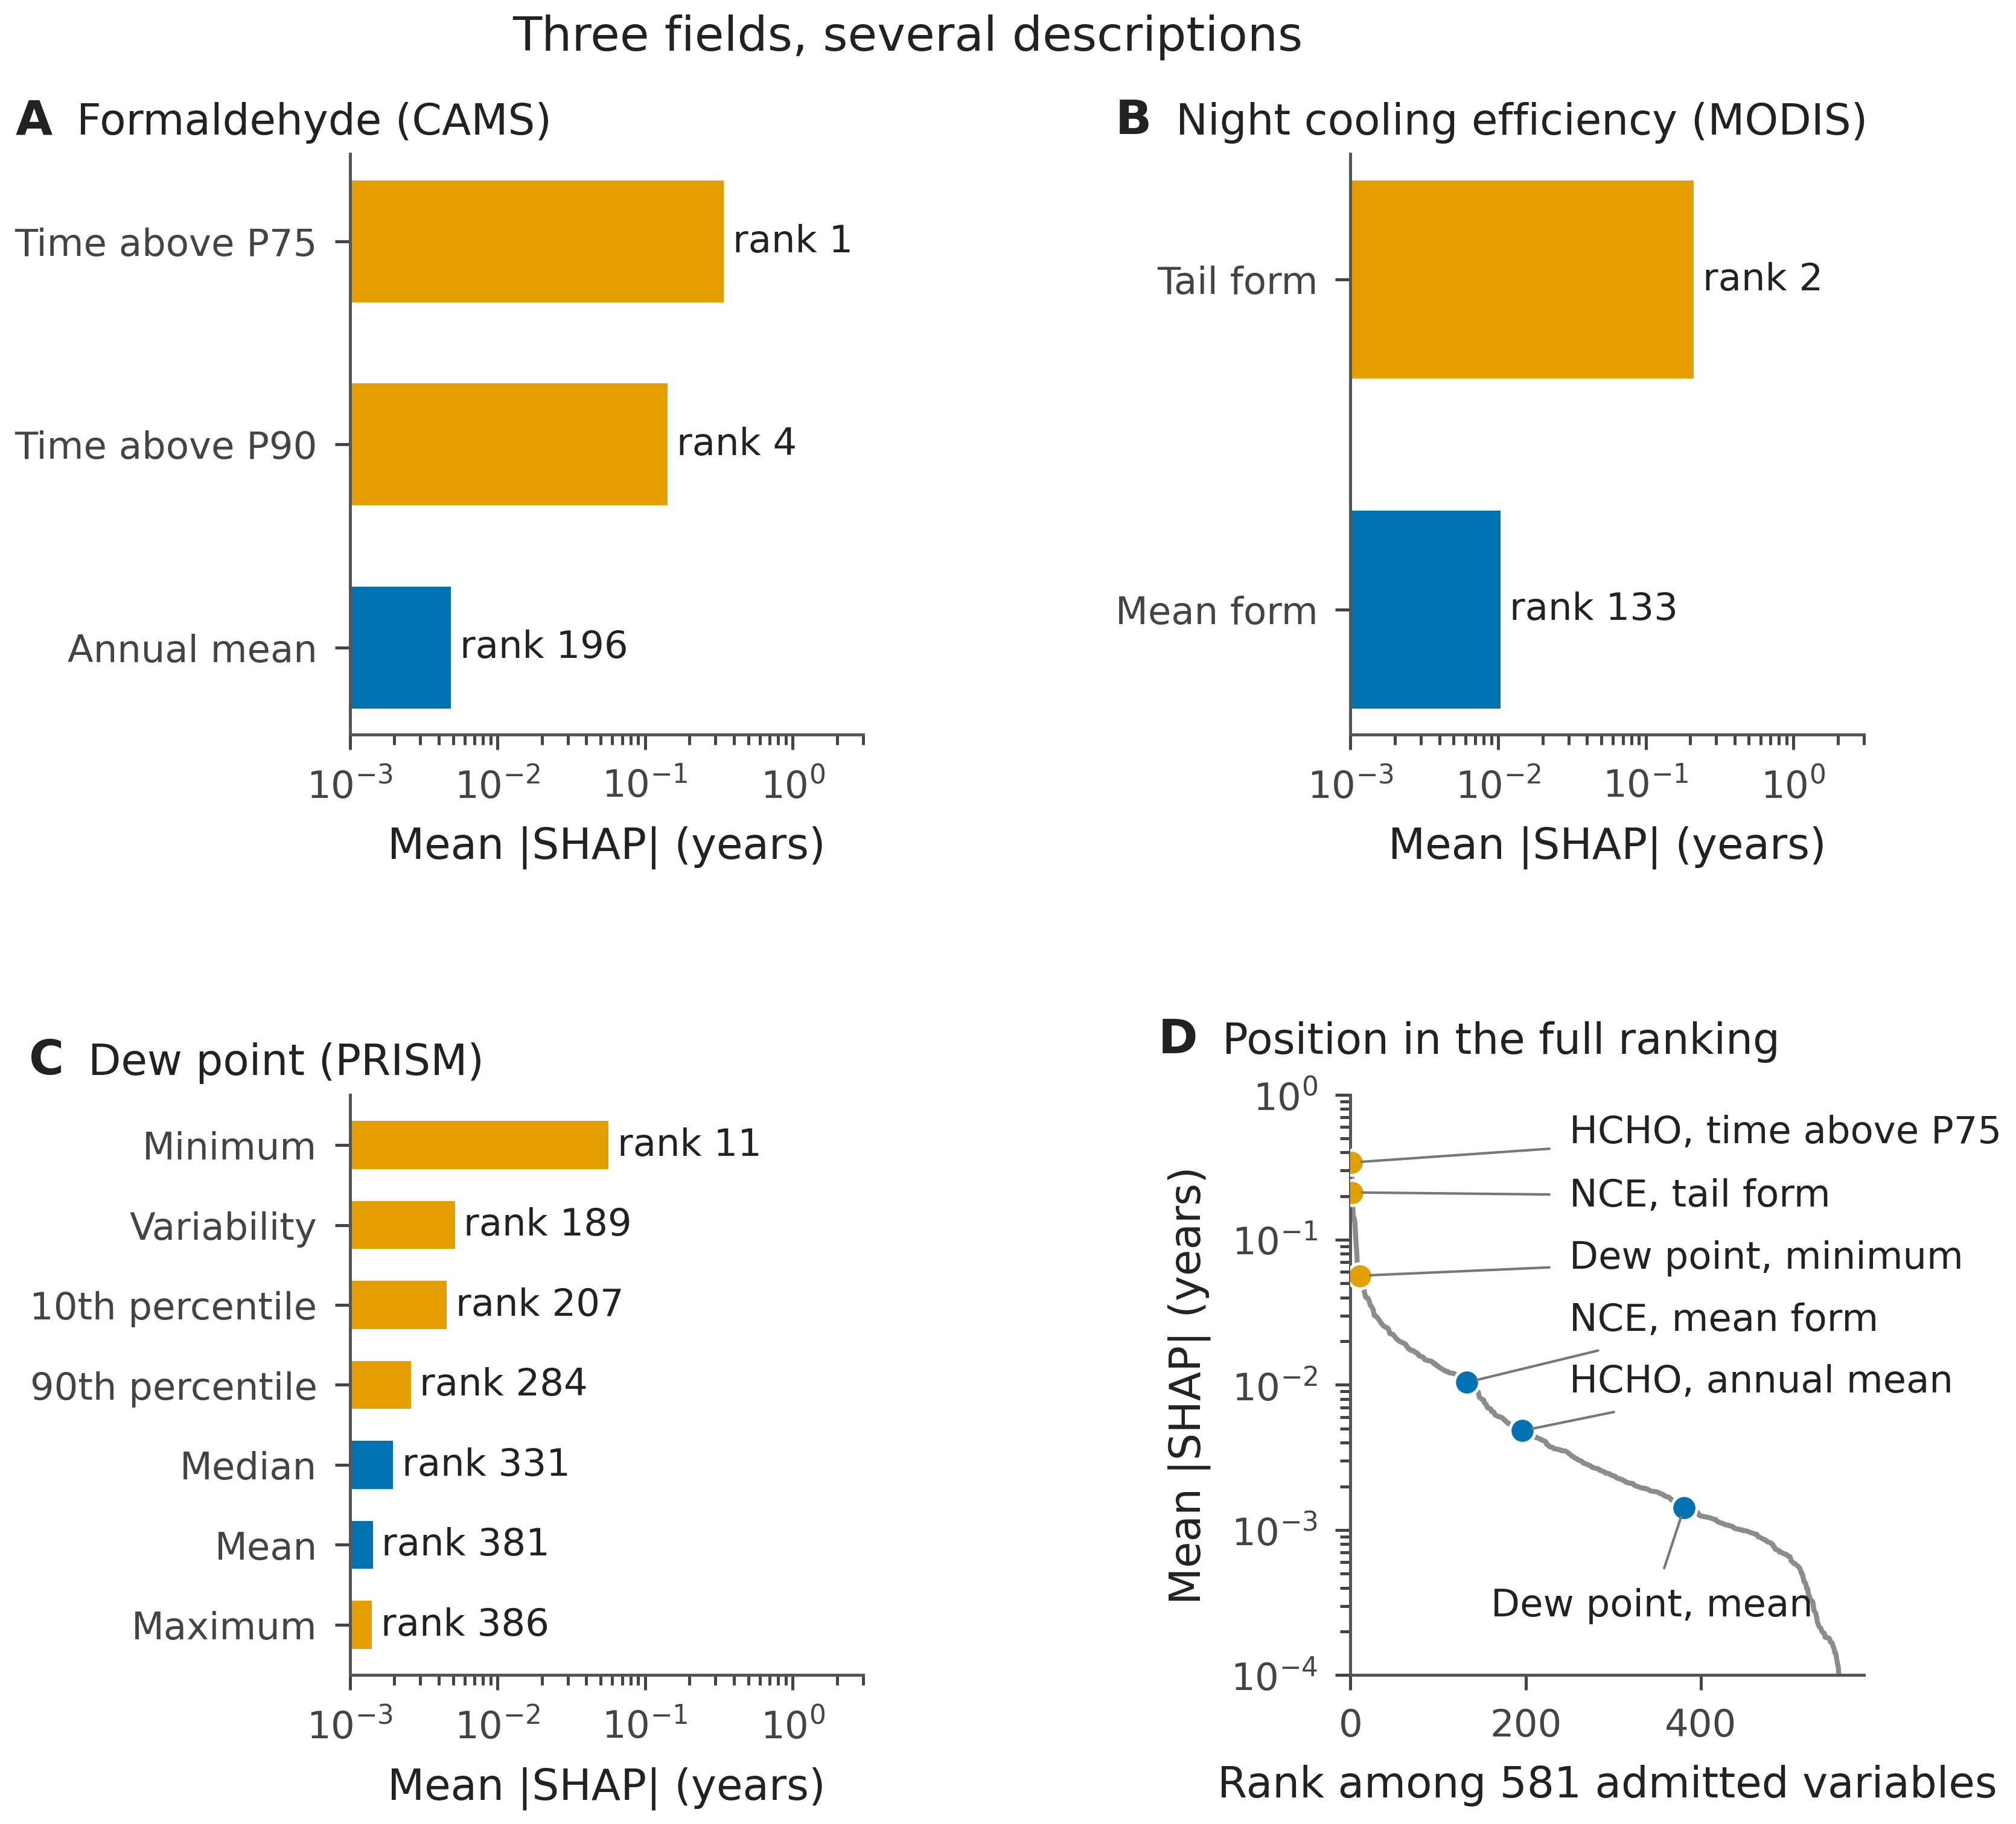
\includegraphics[width=\linewidth]{Figures/Figure03_three_fields.png}
\caption{With the data fixed, the summary chosen for a field sets its
attribution: the formaldehyde time above the 75th percentile ranks first and
the annual mean of the same field \HchoConRank{}th. (A) Out-of-fold mean absolute SHapley
Additive exPlanations (SHAP) value, in years, of three summaries of one
formaldehyde field from the Copernicus Atmosphere Monitoring Service (CAMS),
with their ranks among the \Nfeatpruned{} admitted variables (logarithmic
axis). The summaries are the time above the 75th (P75) and 90th (P90)
percentiles and the annual mean. (B) The same for the tail
and mean forms of night cooling efficiency (NCE) from one satellite
land-surface temperature product, the Moderate Resolution Imaging
Spectroradiometer (MODIS). (C) The same for seven summaries of one
dew-point field from the Parameter-elevation Regressions on Independent Slopes
Model (PRISM), over the cells of each county. Variability is the standard
deviation across those cells. Orange bars are non-central
summaries (time above a level, quantile, extreme, or variability), and blue
bars are central ones (mean or median). (D) The full ranking (grey line), with
the leading and mean summaries marked (HCHO, formaldehyde).}
\label{fig:three}
\end{figure}

Removing the tail form of NCE barely changed skill and passed little of its
attribution to the mean form (Figure~\ref{fig:refit}).
Because the refits (Section~\ref{ssec:m_refit}) are separate fits attributed on their own sample, their
ranks differ slightly from the production ranking. With both present, the tail
form held \RefitFullTailSHAP{} years. With it removed, the mean form's
attribution rose from \RefitFullMeanSHAP{} to \RefitDropMeanSHAP{} years (Figure~\ref{fig:refit}A; rank
\RefitFullMeanRank{} to \RefitDropMeanRank{}, Figure~\ref{fig:refit}B), recovering
\RefitRecoveredPct{}\% of the tail form's attribution. Out-of-fold $R^{2}$ on the second fold set went from
\RefitFullRtwo{} to \RefitDropRtwo{} (Figure~\ref{fig:refit}C). With the mean form removed instead,
skill was \RefitDropMRtwo{} and the tail form ranked first.

Formaldehyde kept the attribution in its other columns. Without the leading duration, the 90th-percentile duration ranked first
and inherited \HchoDropInheritPct{}\% of its attribution (out-of-fold $R^{2}$ on the second fold set,
\HchoDropFullRtwo{} to \HchoDropOneRtwo{}). Without both durations, the annual
means took over the attribution: surface formaldehyde rose from rank \HchoSurfRankWith{}
to \HchoSurfRankWithout{} and total-column formaldehyde from
\HchoColRankWith{} to \HchoColRankWithout{}, and $R^{2}$ fell only to
\HchoDropBothRtwo{}, a loss of \HchoDropBothCost{}. No refit $R^{2}$ has a reported uncertainty. In these refits, the summary decided which column
received the attribution far more than it decided skill.

\begin{figure}[H]
\centering
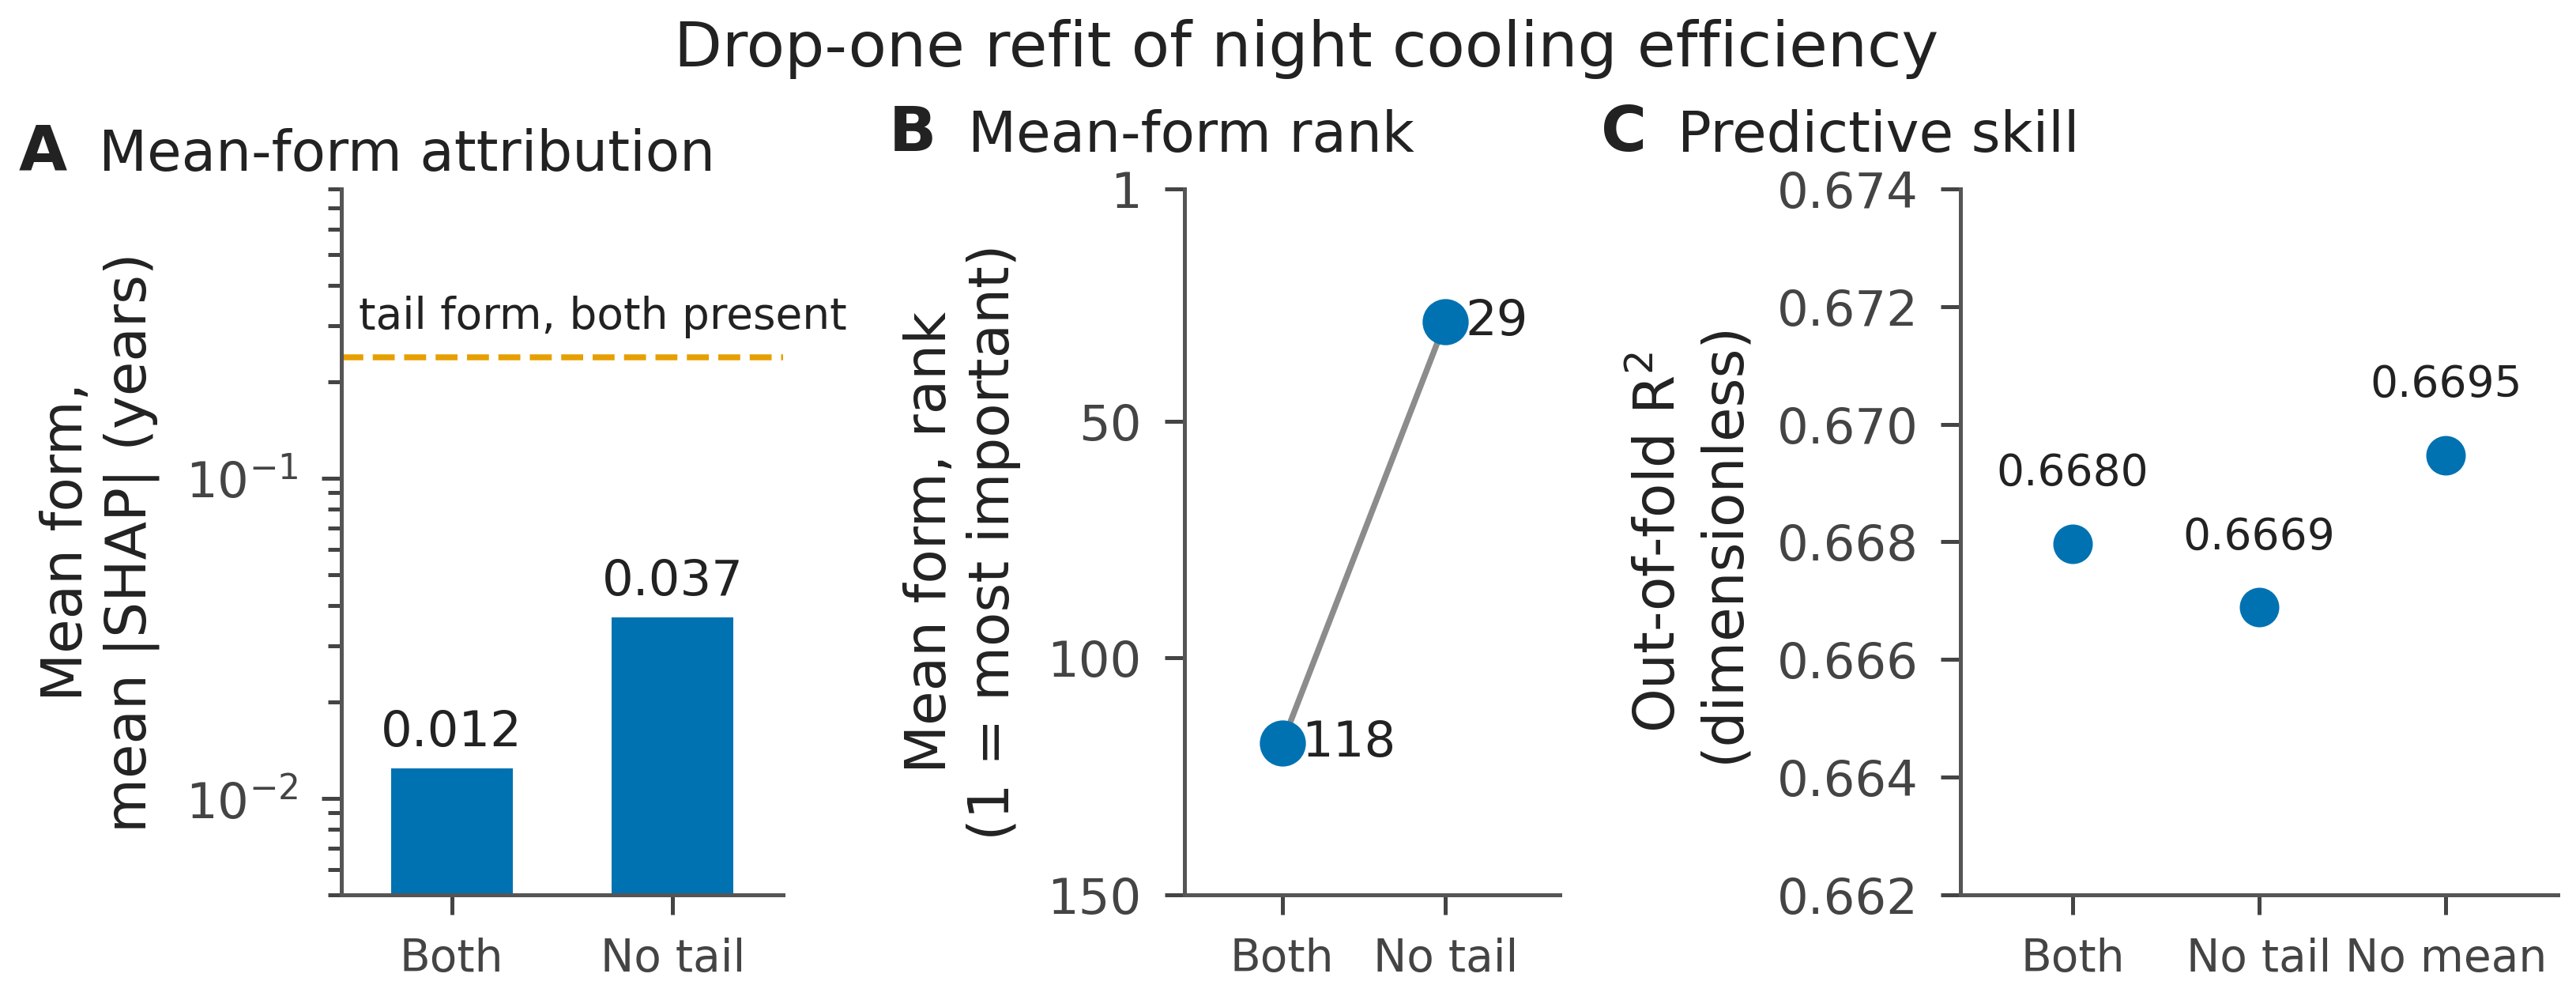
\includegraphics[width=\linewidth]{Figures/Figure04_drop_one_refit.png}
\caption{Removing the tail form of night cooling efficiency (NCE) barely
changes skill and passes only \RefitRecoveredPct{}\% of its attribution to the
mean form. On the horizontal
axes, ``Both'' keeps both forms; ``No tail'' and ``No mean'' remove
that form. (A) Mean absolute
SHapley Additive exPlanations value of the mean form of NCE in the first two
models, over \RefitShapN{} county-years (blue bars); the dashed orange line marks the tail form's own value
with both present (logarithmic axis). (B) The mean form's rank among all
admitted variables in the same two models (blue dots joined by a grey line).
(C) Out-of-fold coefficient of determination ($R^{2}$) of all three models on the second fold set
(blue dots; truncated vertical axis).}
\label{fig:refit}
\end{figure}

\subsection{Atmospheric Composition and Lifetime}
\label{ssec:r_lifetime}
On the second question, with the leading formaldehyde column included, the attribution given to atmospheric
composition (Figure~\ref{fig:composition}A) was concentrated in one family. Oxygenated species
carried \FamOxVOCPct{}\% of it with \FamOxVOCn{} columns, almost all of that from
formaldehyde (\FamHchoPct{}\% from \FamHchoN{} columns), ahead of the
\FamSecondName{} at \FamSecondPct{}\%; no share or ratio here has an interval. For formaldehyde, the time above the
75th percentile carried \HchoPctRatio{}
times the attribution of the time above the 90th; the two correlated at
\HchoDurCorr{}, so the split does not show which level matters
(Section~\ref{ssec:m_attribution}). Across the \PctSpeciesN{} species with both
durations admitted, neither level led consistently (median ratio
\PctSpeciesMedRatio{}; Figure~\ref{fig:composition}B). The 75th percentile led
for \PctSpeciesWins{} of them (formaldehyde, ozone, propane, and sulphur
dioxide). The 90th led for the other four, most widely for
the two sizes of particulate matter, whose 90th-percentile duration carried
\PctPmLo{} to \PctPmHi{} times the attribution of the 75th. Without
formaldehyde, the per-variable advantage of the 75th over the 90th percentile
fell from \PctRatio{}-fold to \PctRatioNoHcho{}-fold.

Atmospheric lifetime broadly tracked whether the model favoured
duration over annual mean concentration (Spearman $\rho$ = \LtRho{}, one-sided
permutation $p$ = \LtPermP{} across \LtSpecies{} species;
Figure~\ref{fig:composition}C,D). Duration carried more attribution for
\LtShortWins{} of \LtShortN{} short-lived species (lifetime under \LtCutoff{}
days; median ratio \LtShortRatio{}) but for only \LtLongWins{} of \LtLongN{}
species persisting \LtCutoff{} days or longer (median ratio \LtLongRatio{}).
The direction held at \LtSweepDirection{} of the \LtSweepN{} class boundaries,
some splitting the species identically; the difference was significant (one-sided Mann--Whitney test, 5\% level; Section~\ref{ssec:m_lifetime}) at only
\LtSweepSig{}, the one fixed in advance. The direction also
held when each species was left out (correlations \LtJackLo{} to \LtJackHi{})
and in \LtValueNegative{}\% of \LtValueDraws{} perturbations of the literature
lifetimes. The relation was consistent in direction and modest in strength.
Formaldehyde, with a lifetime of hours, had the largest ratio; ozone,
peroxyacetyl nitrate, and ethane, the three species that persist for three
weeks or longer, all favoured the mean. Three species in Table~\ref{tab:species}
departed from the ordering: propane and the
reanalysis fine particulate matter, longer-lived but favouring duration, and
isoprene, short-lived with a ratio just below one.

\begin{figure}[H]
\centering
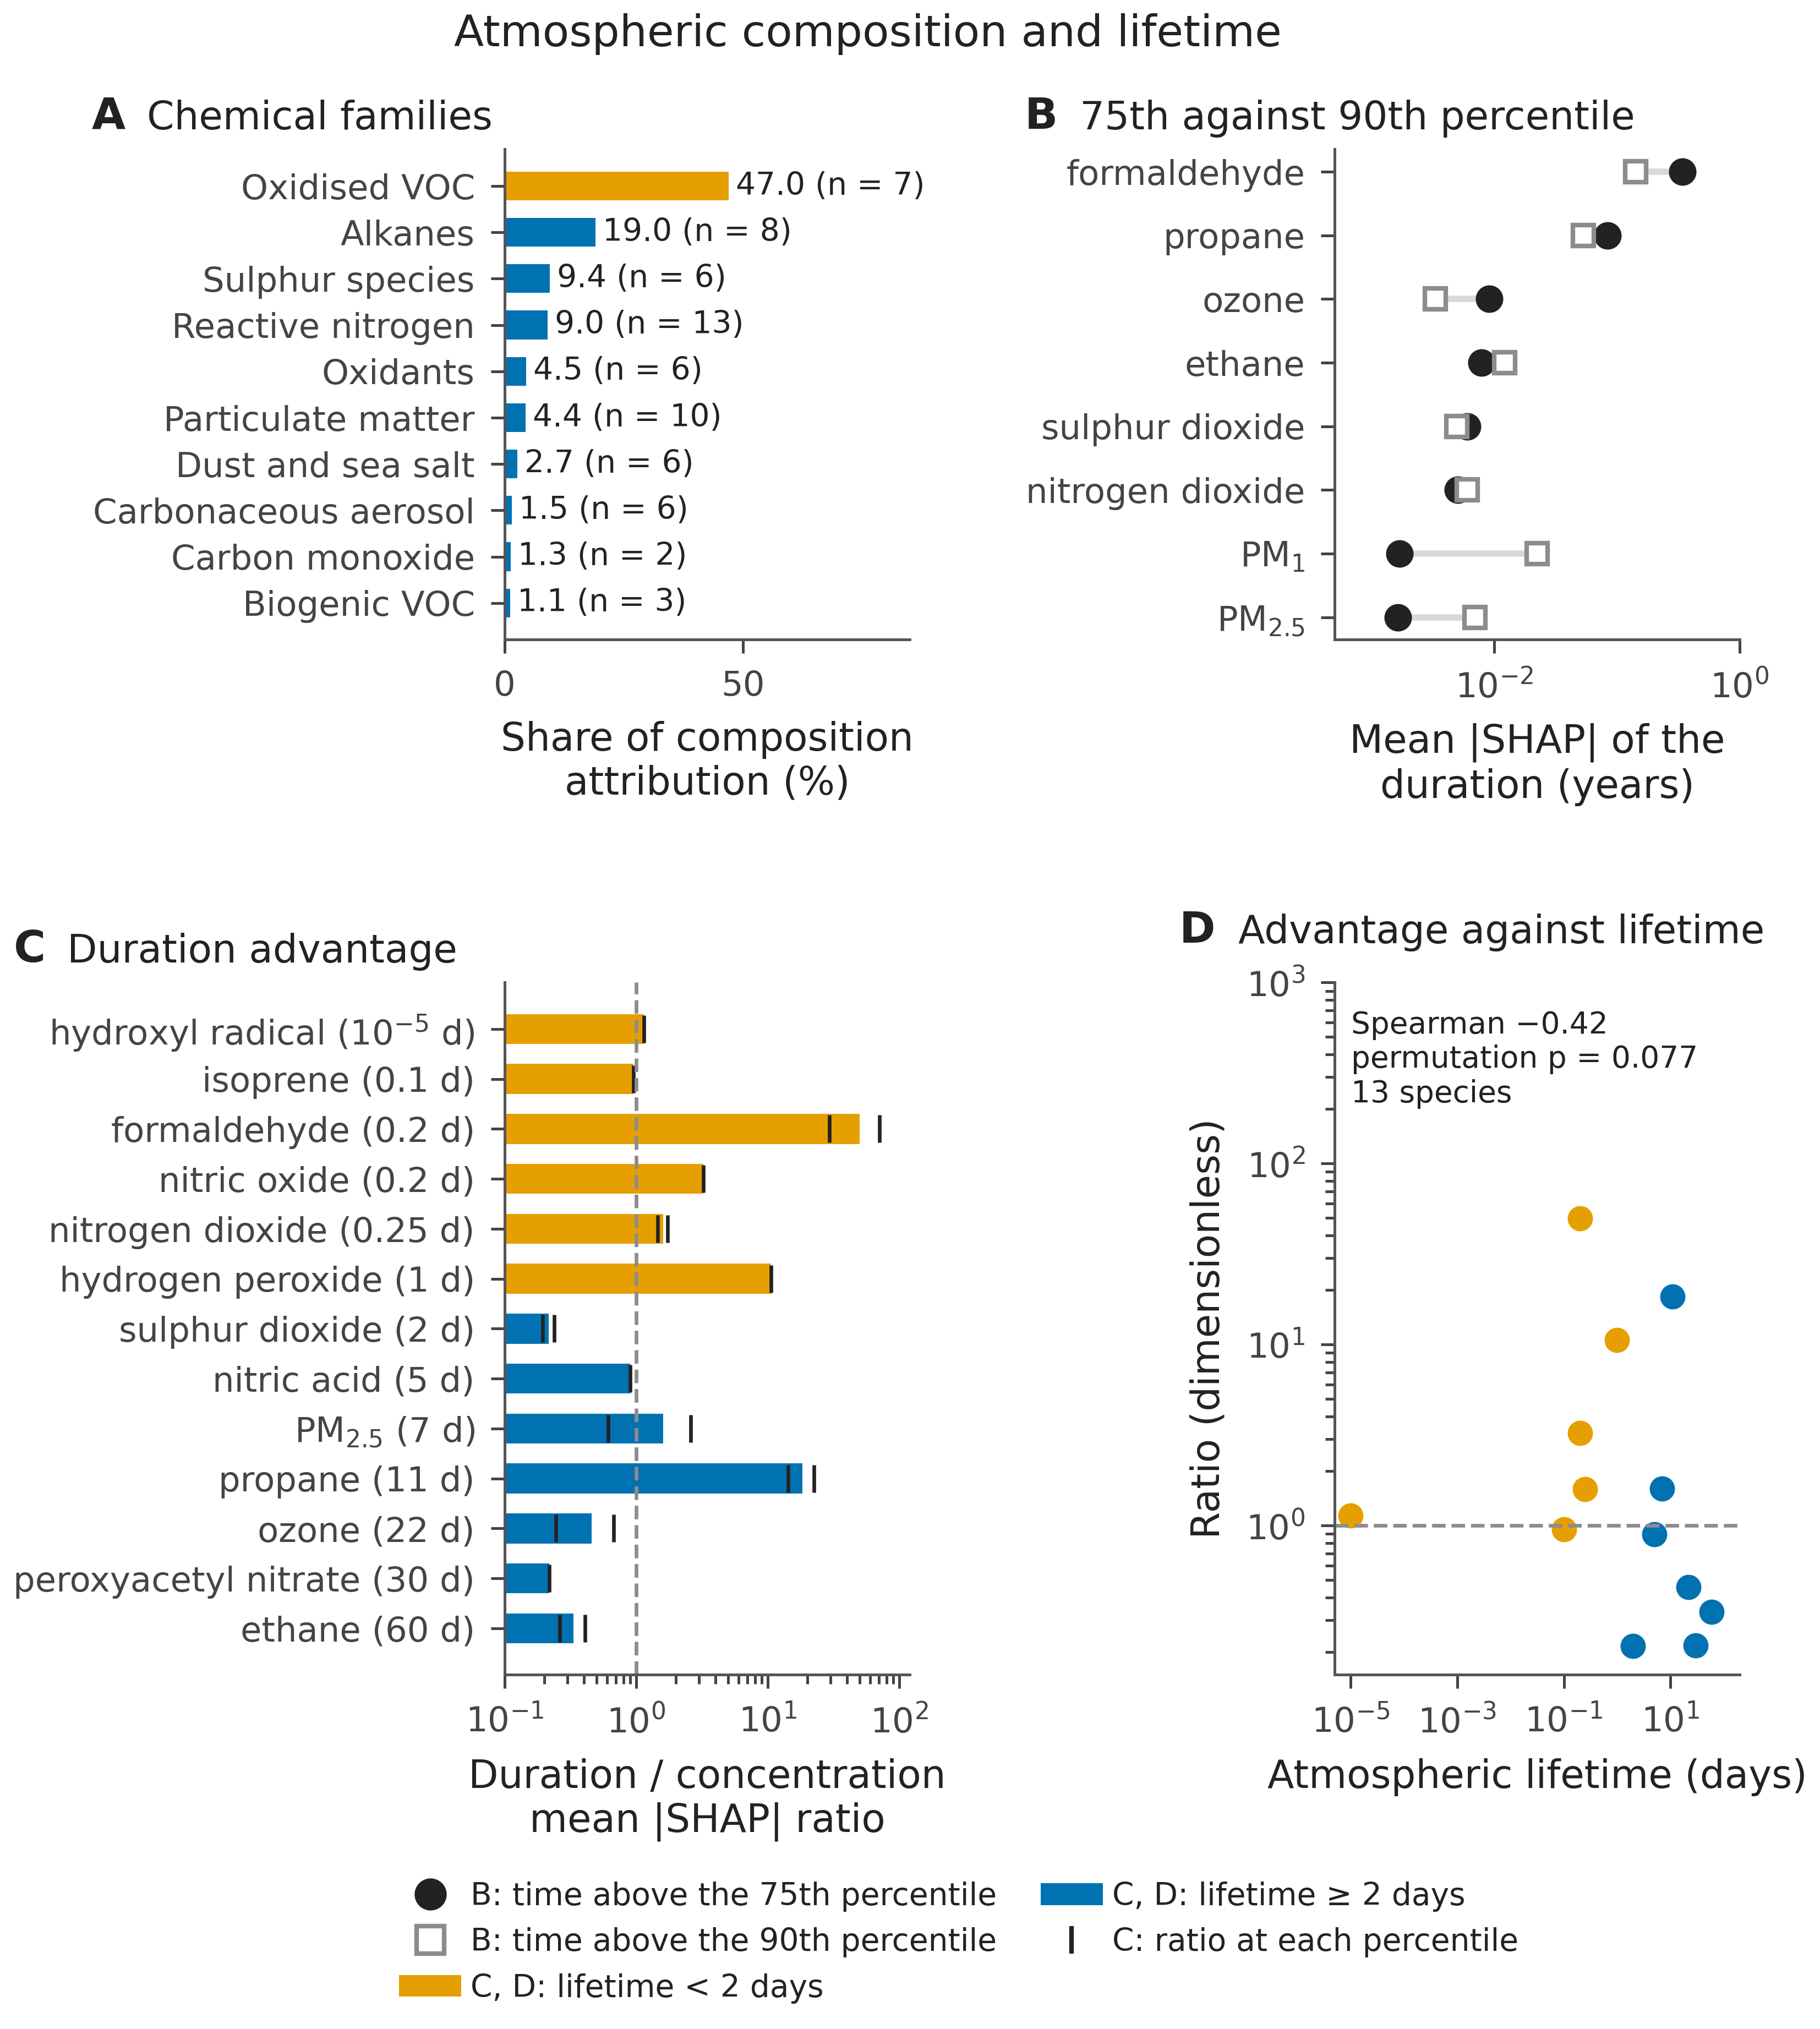
\includegraphics[width=\linewidth]{Figures/Figure05_composition_lifetime.png}
\caption{Of the attribution given to atmospheric composition, formaldehyde
carries the most. The advantage of duration over the annual mean tends to fall
with atmospheric lifetime. (A) Share of the summed out-of-fold mean
absolute SHapley Additive exPlanations (SHAP) value of all \CompN{} composition
columns carried by each chemical family, with the number of columns ($n$);
VOC, volatile organic compounds. Oxidised VOC, the
oxygenated species: formaldehyde and hydrogen
peroxide. (B) Mean absolute SHAP value of each species'
time above the 75th percentile (black circles) and above the 90th (open
squares), joined by a grey line (logarithmic axis). PM$_{1}$ and PM$_{2.5}$,
reanalysis particulate matter with an aerodynamic diameter of at most 1 and 2.5
micrometres. (C) Median ratio of the
duration to the concentration importance for each species, ordered by
atmospheric lifetime in days (d, in brackets; logarithmic axis). Orange bars
mark lifetimes under \LtCutoff{} days, blue bars \LtCutoff{} days or longer, black ticks the
ratio for each duration percentile, and the dashed line equal importance.
Lifetime
is the tropospheric burden divided by the removal rate, an e-folding time, not
a half-life. (D) The same ratio against lifetime, one dot per species in the
same colours, with the Spearman rank correlation and its permutation $p$
value.}
\label{fig:composition}
\end{figure}

\subsection{Turning Points of the Attribution Curves}
\label{ssec:r_turning}
On the third question, under the stability criterion of
Section~\ref{ssec:m_turning}, \TpStable{} of the \TpTotal{} candidate turning points passed.
Three describe moisture and
night cooling (Figure~\ref{fig:curves}, Table~\ref{tab:turning}). The minimum dew point turned at \TpDew{}\,\textdegree C (95\%
interval \TpDewLo{} to \TpDewHi{}), the night-time wet-bulb temperature at
\TpWet{}\,\textdegree C (\TpWetLo{} to \TpWetHi{}), and the tail form of NCE at
\TpNce{} (\TpNceLo{} to \TpNceHi{}). These intervals
(Figure~\ref{fig:stability}A) were narrow; the widest covered
\TpTripletWidthMax{}\% of its range. Every interval is likely too narrow
(Section~\ref{ssec:m_turning}).
Each crossing lay near the middle of its
variable's distribution,
with \TpDewAbove{}\%, \TpWetAbove{}\%, and
\TpNceAbove{}\% of county-years above the three values, as expected even for a monotone curve (Section~\ref{ssec:m_turning}). Each therefore
marks a
change of sign, not necessarily a change in slope. Above their
turning points, the minimum dew point and the night-time wet-bulb temperature
lowered the model's prediction, and NCE raised it
(Figure~\ref{fig:curves}A--C). Because NCE also rises in cooler climates (Section~\ref{ssec:m_descriptions}), the
higher prediction above \TpNce{} may reflect a cooler county, not only stronger
cooling. The night-time wet-bulb curve spanned a smaller range of
attribution than the dew-point and night-cooling curves (Figure~\ref{fig:curves}A--C), so its turning point
was well located but moved the prediction less.

Two composition variables also passed. The formaldehyde duration turned at
\TpHcho{}\% of the year (95\% interval \TpHchoLo{} to \TpHchoHi{}) and the
ratio of formaldehyde to nitrogen dioxide at \TpRatio{} (\TpRatioLo{} to
\TpRatioHi{}). Of county-years, \TpHchoAbove{}\% and \TpRatioAbove{}\% lay
above these two values. Above both, the attribution was
negative (Figure~\ref{fig:curves}D,E). The ratio is formed from reanalysis
fields, not the satellite columns for which its regime thresholds were
derived~\cite{Duncan2010}, so its turning point cannot be read on that scale.
Its curve spanned less attribution than those in panels A, C, and D (Figure~\ref{fig:curves}E).

Of the other six candidates (Table~\ref{tab:turning}), four passed outright:
the mean form of
NCE, the warm-hour wet-bulb temperature, the minimum temperature, and
the share of cropland in corn. Mean night-time LST failed: its
full-sample crossing at \TpLst{}\,\textdegree C lay outside its own bootstrap
interval. Annual mean satellite-derived PM$_{2.5}$ met the criterion only
formally, with the
widest interval (\TpPmWidth{}\% of its range) and the full-sample value near
its lower edge, so we do not interpret it. Neither numerical limit decided any
candidate: a crossing was found in every resample, where 60\% suffice, and
every interval was narrower than 40\% of its range.

\begin{figure}[H]
\centering
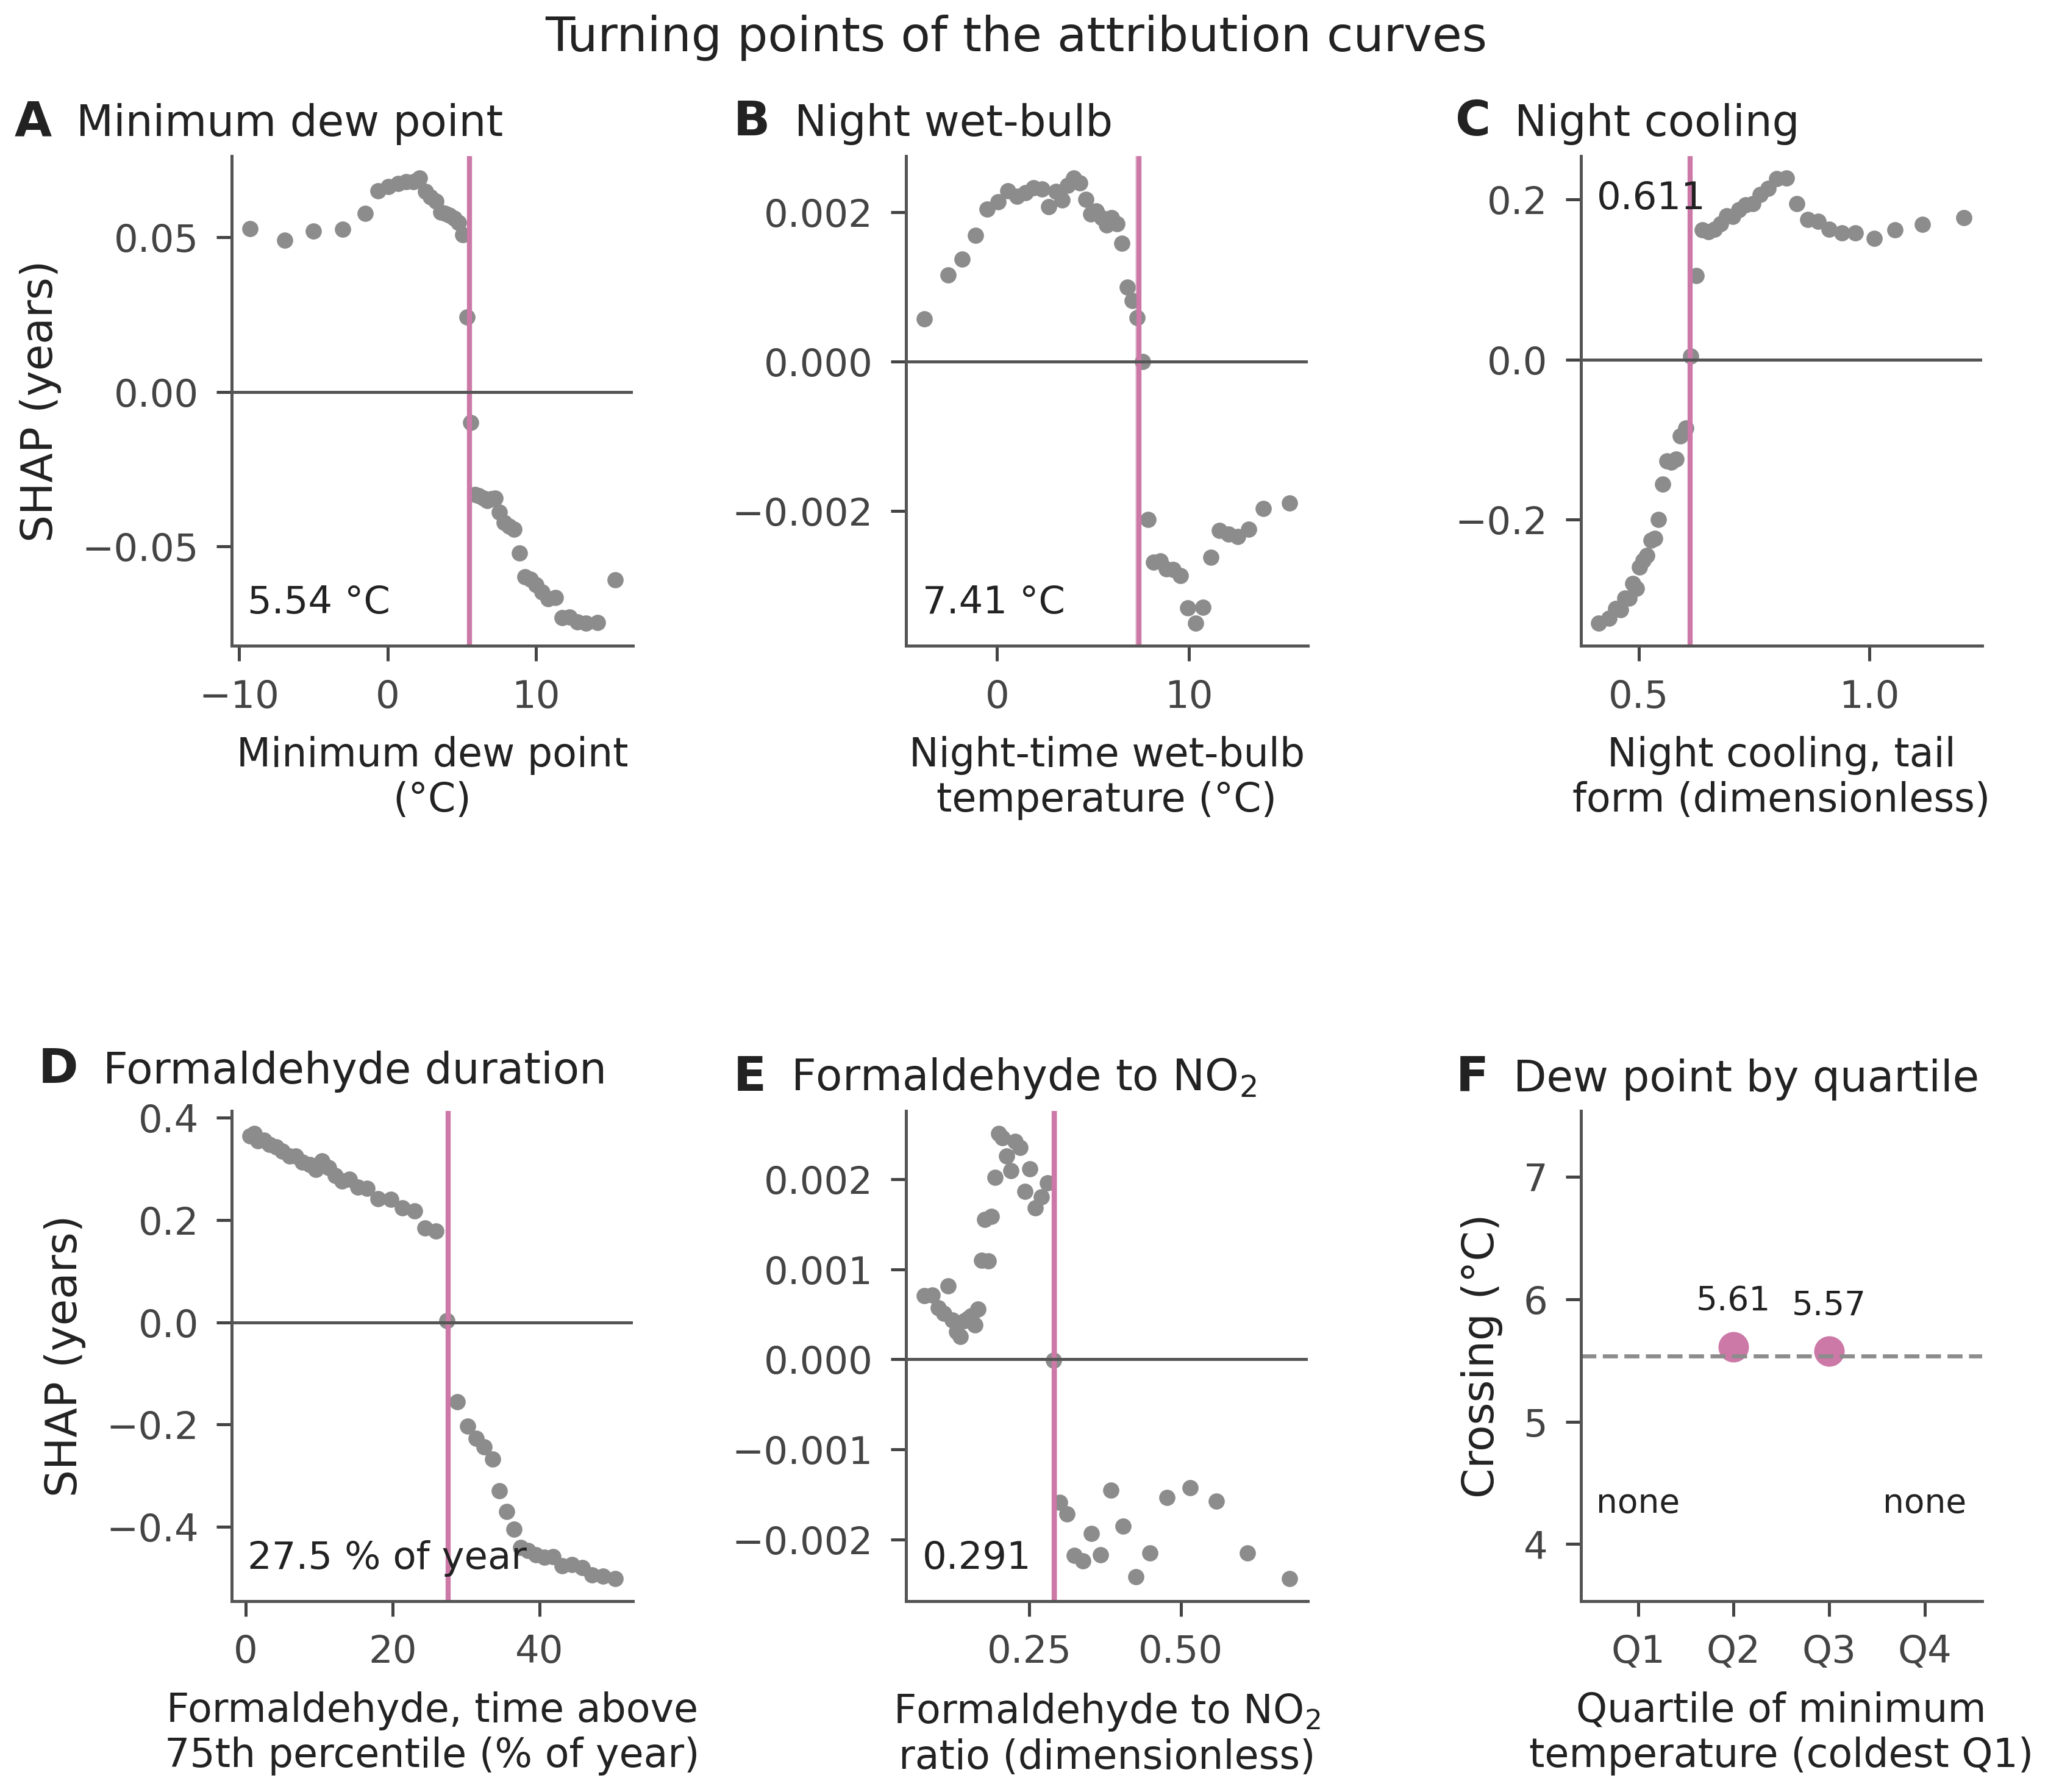
\includegraphics[width=\linewidth]{Figures/Figure06_turning_point_curves.png}
\caption{Five attribution curves change sign within a narrow bootstrap
interval of one fitted model. (A to E) Median SHapley
Additive exPlanations (SHAP) value, in years, of \GateShapN{} county-years in 45 equal-count bins (grey
dots) against the minimum dew point, the night-time
wet-bulb temperature, the tail form of night cooling efficiency, the
formaldehyde time above the 75th percentile, and the ratio of formaldehyde to
nitrogen dioxide (NO$_2$). The
vertical scales differ: the curves in B and E span less attribution than
those in A, C, and D. The pink line is the located turning point; its 95\%
bootstrap interval (Table~\ref{tab:turning}) is too narrow to show.
(F) The dew-point turning point located within each quartile of the minimum
temperature (Q1 coldest); it appears only in the two middle quartiles,
and the dashed line is the value for all county-years.}
\label{fig:curves}
\end{figure}

\subsection{Stability of the Turning Points}
\label{ssec:r_invariance}
No null yielded a stable turning point. With attribution permuted
against its predictor \NullCrossDraws{} times for each of the \TpTotal{}
candidates, the procedure passed the criterion in \NullCrossPasses{} of
\NullCrossTotal{} runs (Figure~\ref{fig:stability}B). For most candidates, no
permuted curve crossed zero. On curves raised until
no crossing existed, the procedure passed for \NullCrossShifted{} of the
\TpTotal{} candidates.

Over \PertDraws{} draws per level, noise of 1\% of a predictor's standard deviation shifted all \TpTotal{} candidates by a
median of \PertOneMed{} interval widths, and noise of 5\% by \PertFiveMed{}.
Only at 10\% did the median shift reach \PertTenMed{} and the largest exceed
one width (\PertTenMax{}; Figure~\ref{fig:stability}D). The noise is
independent random error; the spatially correlated errors of the products,
such as clear-sky sampling and reanalysis bias, were not simulated.

Within the one fitted model, the three turning points of moisture and night
cooling moved by at most \RegMerTripletMax{}\% of their range when split by region
(Figure~\ref{fig:stability}C). Split at the 100th meridian, the sample held
\RegMerWest{} attributed county-years in the drier west and \RegMerEast{} in
the east (Section~\ref{ssec:m_turning}). The turning points for minimum
dew point and night-time wet-bulb temperature
drifted by \RegMerDewAbs{} and
\RegMerWetAbs{}\,\textdegree C. The western half also lies on higher
ground, where the Stull formula overstates the wet-bulb temperature (Section~\ref{ssec:m_data}). At the 100th meridian, the minimum dew point
and the tail form of NCE shifted by \RegMerDew{}\% and \RegMerNce{}\% of their
range, more than their own 95\% interval widths (\TpDewWidth{}\% and
\TpNceWidth{}\%; Figure~\ref{fig:stability}A). At the median longitude, the
largest shift was \RegMedTripletMax{}\%, and the dew-point and wet-bulb turning points drifted by \RegMedDewAbs{}
and \RegMedWetAbs{}\,\textdegree C.

The split moved some turning points. At the 100th meridian, mean night-time LST
moved by \RegMerLst{}\% and satellite-derived PM$_{2.5}$ by \RegMerPm{}\% of
their
range, and the mean form of NCE had no crossing west of it. At the median
longitude, the ratio of formaldehyde to nitrogen dioxide moved by
\RegMedRatio{}\% of its range.

Stability under the split was not unique to the
three moisture and night-cooling variables. Minimum temperature
(\RegMerTmin{}\% of its range at the 100th meridian), the formaldehyde
duration, and the share of cropland in corn also moved little (Figure~\ref{fig:stability}C).

The raw
minimum dew point and minimum temperature correlated at \RawCorr{}, but their
attributions correlated at only $r$ = \ShapCorr{} (no interval reported), suggesting that one turning point
is not a copy of the other. Within quartiles of the
minimum temperature (Figure~\ref{fig:curves}F), the dew-point crossing
appeared in \StrataWithCrossing{} of \StrataTotal{}, the temperate middle, at
\StrataCrossLo{} and \StrataCrossHi{}\,\textdegree C.
%

\begin{figure}[H]
\centering
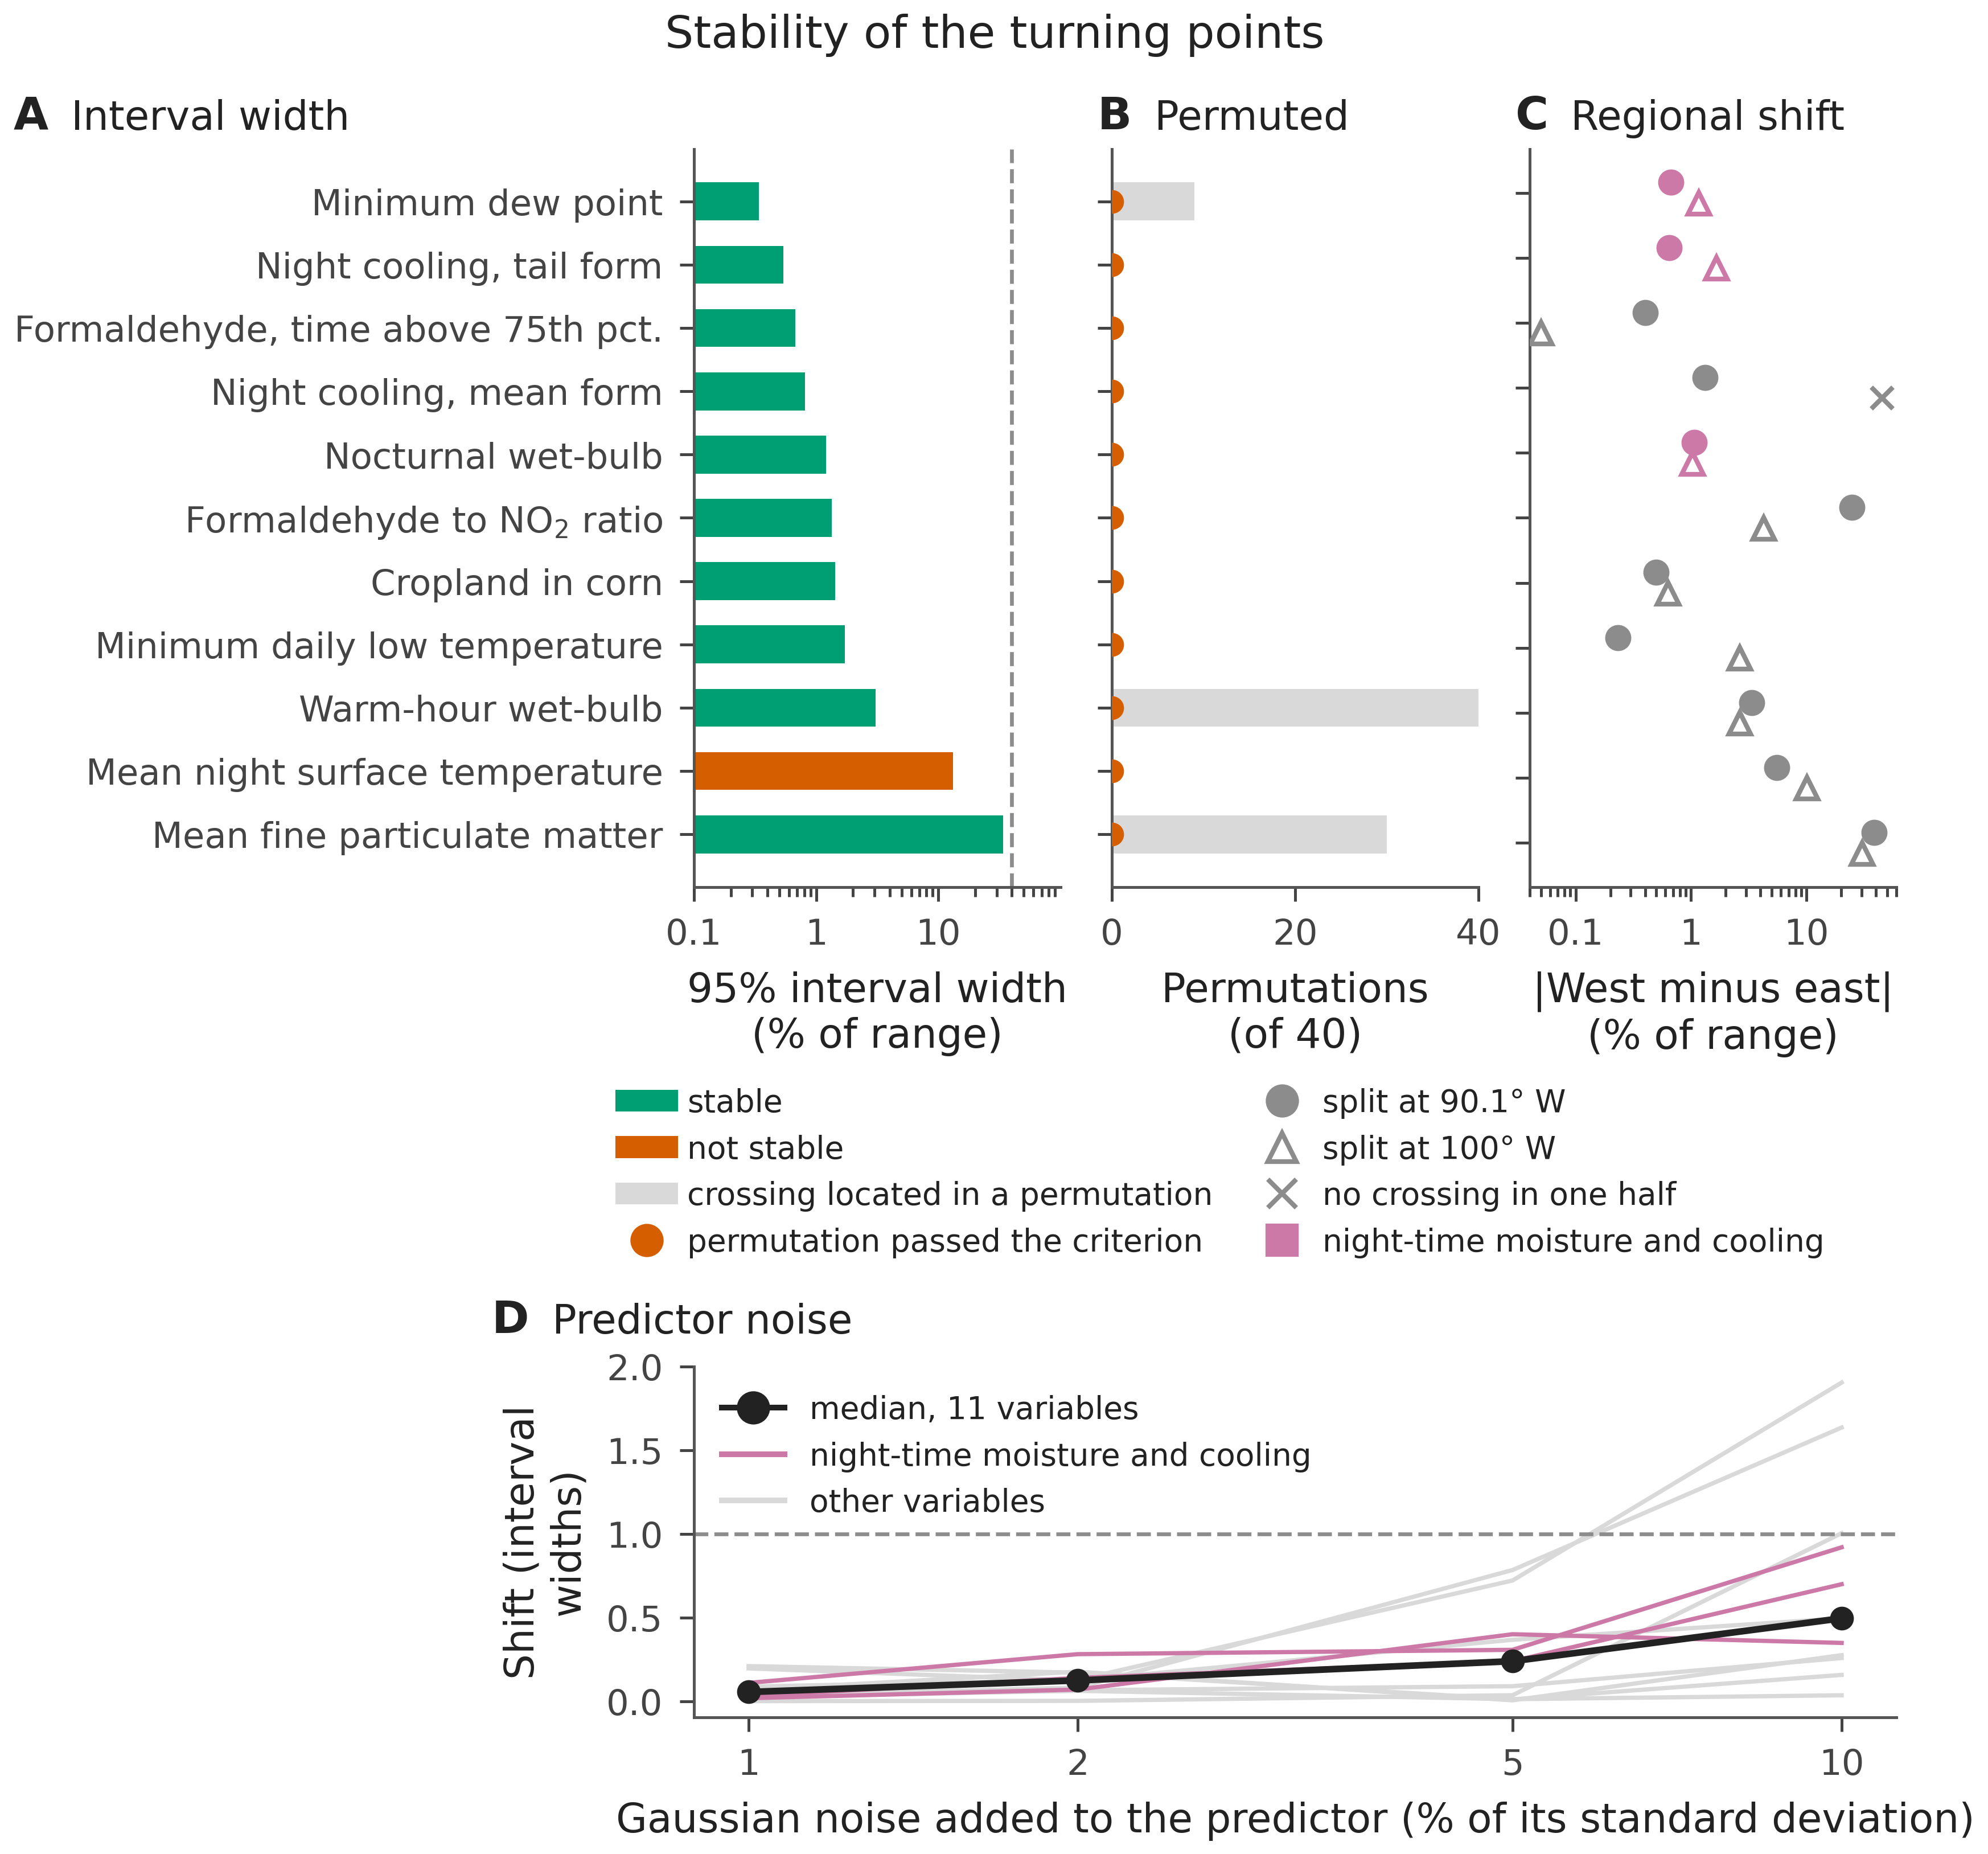
\includegraphics[width=\linewidth]{Figures/Figure07_turning_point_stability.png}
\caption{Of the \TpTotal{} candidate turning points, \TpStable{} pass the
stability criterion and no permuted curve does. Across
the 100th meridian, the three moisture and night-cooling turning points move
by at most \RegMerTripletMax{}\% of their range. (A) Width of the 95\%
bootstrap interval (\TpBoot{} resamples) of each turning point as a share of the variable's
range (logarithmic axis). Green bars pass the stability criterion, and the
dashed line is the 40\% limit. (B) The same procedure on attributions
shuffled \NullCrossDraws{} times against their own variable: grey bars count shuffles in which a
crossing was found, and orange dots those that passed the criterion (all
zero). (C) Absolute west minus east shift of each turning point as a share of
its range, with the country split at the 100th meridian (triangles)
and at its median longitude (circles; logarithmic axis). A cross marks a
variable with no crossing in one half, and pink marks the three moisture and
night-cooling variables (minimum dew point, night-time wet-bulb temperature,
tail form of night cooling efficiency). (D) Shift of each turning point, in
interval widths, when noise of 1 to 10\% of the variable's standard deviation
is added. Pink lines are those three variables, and
the black line is the median of all \TpTotal{}. PM$_{2.5}$, satellite-derived particulate matter
with an aerodynamic diameter of at most 2.5 micrometres; NO$_2$, nitrogen
dioxide.}
\label{fig:stability}
\end{figure}

\subsection{Model Error and Socioeconomic Conditions}
\label{ssec:r_failure}
On the fourth question, the model's error (Figure~\ref{fig:failure}A) was geographically structured.
County mean residuals had a standard deviation of \ResSD{} years and were
weakly but significantly clustered (Moran's $I$ = \ResMoranI{}, $p$ =
\ResMoranP{}, against \ResMoranOutcome{} for life expectancy). The model overpredicted life expectancy by \ResMissYears{}
years or more in \ResMissN{} counties, most of them in the northern Plains
(South Dakota, North Dakota, and Montana), the interior West and Southwest, and
Virginia. Among them, the Virginia units, Baltimore, St.\ Louis, and Carson
City are independent cities; each draws its reanalysis values from the
same grid cells as its neighbours.

The \ResSdohN{} socioeconomic columns that never entered the model, averaged over \ResSdohYearLo{} to \ResSdohYearHi{} only, predicted
the county residual out of fold with $R^{2}$ = \ResSdohRtwo{} under folds
grouped by state. Part of this signal may enter through the outcome's covariates (Section~\ref{ssec:m_outcome}). The
\ResEnvN{} environmental columns the model had
used gave \ResEnvRtwo{}, no better than the mean (Figure~\ref{fig:failure}B).
The socioeconomic result does not rest on the
health-behaviour columns: without the County Health Rankings, the
socioeconomic columns gave $R^{2}$ = \ResNoChrRtwo{}, and the American
Community Survey columns alone gave \ResAcsRtwo{}. None of these $R^{2}$ values has an interval. All six indicators named in advance, each taken alone,
were correlated with the residual in the expected direction (Figure~\ref{fig:failure}C).
Absolute Spearman correlations ran from \ResAbsRhoLo{} to \ResAbsRhoHi{} (largest
Holm-corrected $p$ = \ResHolmMax{}, too small because counties were treated as independent; Section~\ref{ssec:m_sdoh}). The model
overpredicted where poverty, unemployment, uninsurance, and disability were high and
underpredicted where income and education were high.

\begin{figure}[H]
\centering
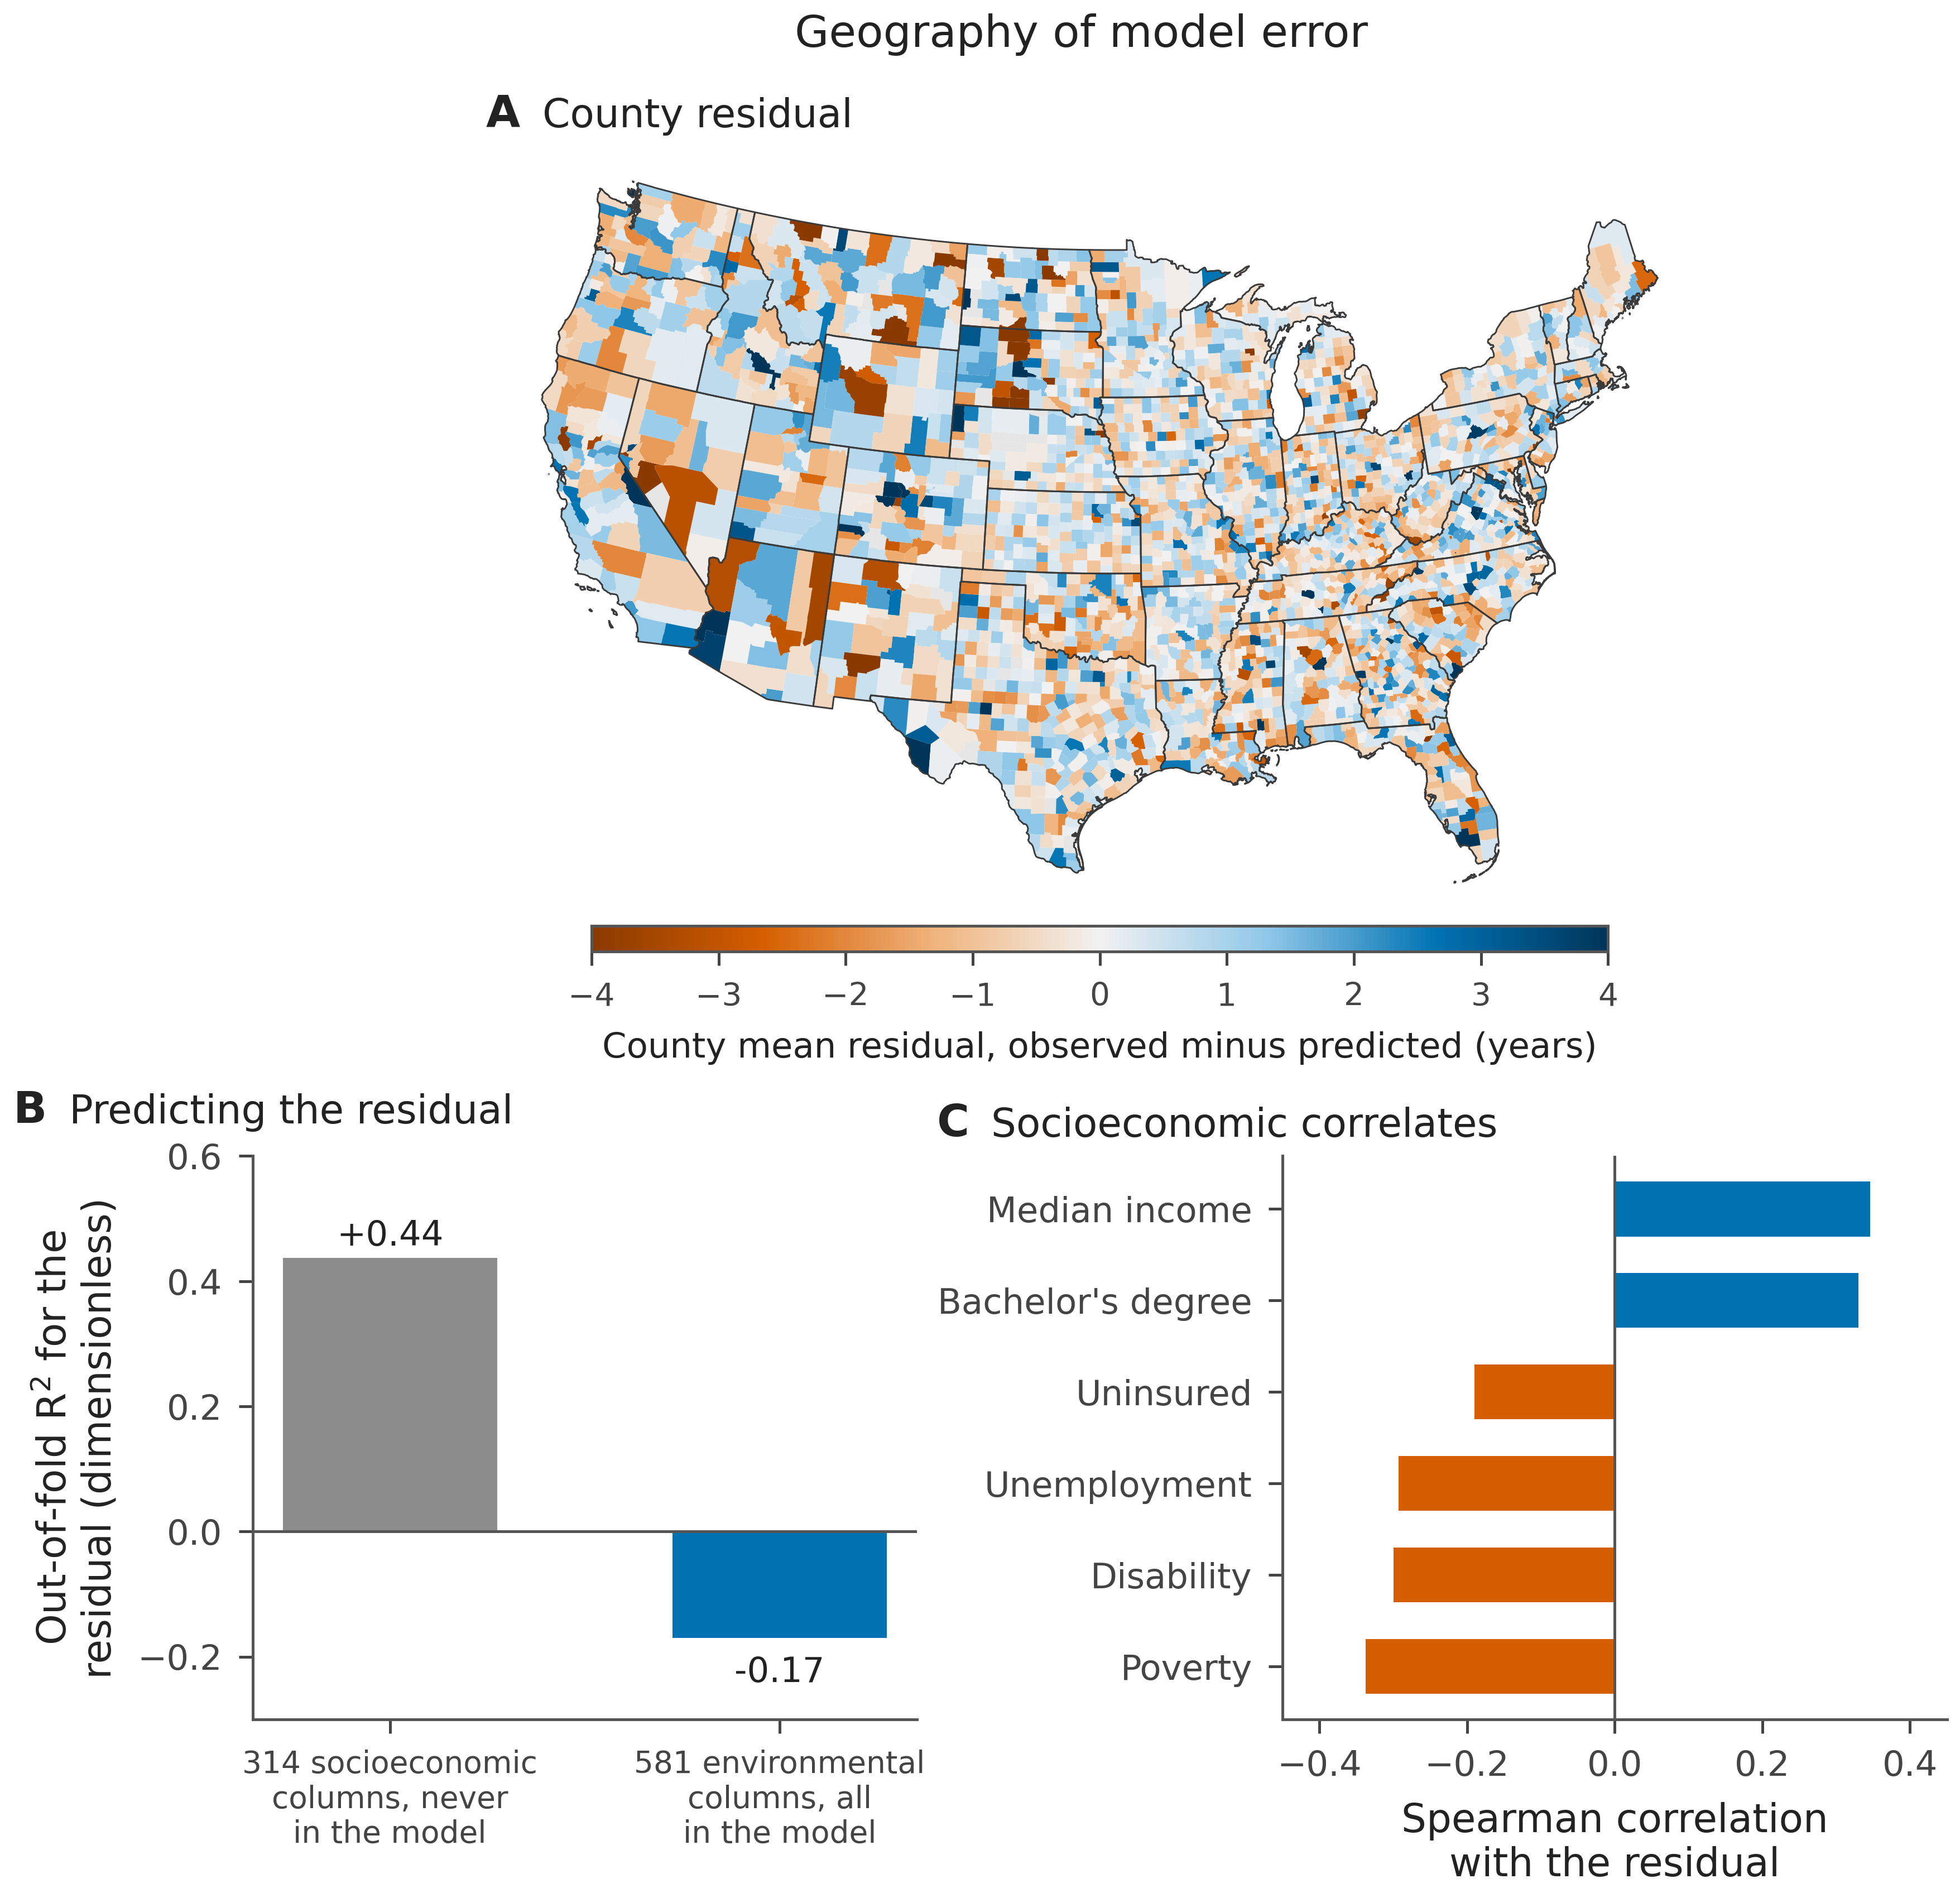
\includegraphics[width=\linewidth]{Figures/Figure08_failure_geography.png}
\caption{Socioeconomic variables the model never saw predict its error; its own
environmental inputs do not. (A) County mean out-of-fold residual of \Ncounties{} counties,
observed minus predicted life expectancy over \YearStart{} to \YearEnd{}:
orange counties have lower life expectancy than the model predicts, and blue
counties higher; thin lines are state boundaries. (B) Out-of-fold coefficient
of determination ($R^{2}$) for predicting the county residual, with folds
grouped by state, from the \ResSdohN{} socioeconomic columns kept out of the
model (grey bar). The blue bar uses the \ResEnvN{} environmental columns in it.
(C) Spearman correlation of the residual with six indicators named in
advance: blue bars positive, orange bars negative.}
\label{fig:failure}
\end{figure}

%% ======================================================================
\section{Discussion}
\label{sec:discussion}
With the data held fixed, the summary chosen for a field moved its attribution
far more than the model's skill, a dependence our earlier
rankings~\cite{Ruwali2026multi, Ahmad2026night, Shrestha2026exp} left untested.
Formaldehyde's leading duration (its time above a level), chosen post hoc, carried \HchoRatio{} times the attribution of
its annual mean (no interval), perhaps partly by construction (Section~\ref{ssec:d_limits}); across \StatFieldsTotal{} other fields, the most and least attributed summaries differed by a median factor of
\CensusMedianSpread{}; and a drop-one refit of night cooling moved the ranking while $R^{2}$ went
only from \RefitFullRtwo{} to \RefitDropRtwo{} (Section~\ref{ssec:r_two}). Whether the model favoured duration or
the mean tracked atmospheric lifetime only weakly (one-sided
$p$ = \LtPermP{}). Of \TpTotal{} candidate turning points, values where a variable's attribution
changes sign, \TpStable{} met a
stability criterion fixed in advance, as properties of one fitted model.
Socioeconomic variables the model never saw predicted its error (out-of-fold $R^{2}$ =
\ResSdohRtwo{}).

\subsection{What an Attribution Ranking Measures}
\label{ssec:d_rashomon}
A high rank shows that the model routes its prediction through an input, not
that the input adds skill no other holds. Without its favoured summary a
field can fall far, as night cooling did to \RefitDropMeanRank{}th, or stay
first, as formaldehyde did through its 90th-percentile duration (Section~\ref{ssec:r_two}).

Refits without a whole data block
(Section~\ref{ssec:r_model}) also separate rank from skill: the 90th percentile and mean of soil bulk
density, a static map, ranked \SoilPninetyRank{}th and \SoilMeanRank{}th, yet
removing the soil block did not lower skill. Equally accurate models can
rank inputs differently, the Rashomon effect~\cite{Breiman2001two}, so
the importance of a variable is better read as a range over such models than
as its value in one~\cite{Fisher2019, Dong2020}. Grouped attribution of a field's summaries
avoids dividing attribution among correlated summaries but cannot set one summary against the
rest~\cite{Au2022}. Epidemiology met the same equivalence for heat: across 107 United
States cities, mean, minimum, maximum, and apparent temperature predicted
mortality about equally well, and no measure was best
everywhere~\cite{Barnett2010}. Only a refit tells which summary the model needs.

\subsection{Atmospheric Composition and Lifetime}
\label{ssec:d_physics}
Where the summary matters, the model's preference followed chemistry in
direction, though weakly. The oxygenated family, chiefly formaldehyde, led the
composition attribution
(Section~\ref{ssec:r_lifetime}). Among the
187 hazardous air pollutants on the United States Environmental Protection
Agency's list in 2017, a list that excludes ozone and particulate matter,
formaldehyde is the most important carcinogen in outdoor air~\cite{Zhu2017}.
In China, daily ambient formaldehyde was associated with nonaccidental
mortality in 275 counties~\cite{Ban2022}, and long-term tropospheric
formaldehyde columns with respiratory mortality in 466 counties and
districts~\cite{Yu2024}.
For formaldehyde, the 75th-percentile duration may
track the length of the warm season of isoprene
oxidation~\cite{Millet2008}; if so, the leading variable is better read as a
marker of persistent warm-season photochemistry than as a measured exposure.
Because no socioeconomic variable entered the model directly
(Section~\ref{ssec:m_design}), the duration can also
carry the social geography of counties with a long warm season. The variable
is also a model field, not a retrieval, from the CAMS reanalysis, the coarsest
product in the model, whose grid cells are wider than most counties
(Table~\ref{tab:data}). Part of its attribution can therefore reflect regional
position rather than county conditions, as location-like predictors
can~\cite{Meyer2019}.

Across species, the preferred summary tended to follow a broad chemical order
(Spearman $\rho$ = \LtRho{}, one-sided $p$ = \LtPermP{},
\LtSpecies{} species):
duration was favoured for species destroyed within hours and the mean for
species that persist for weeks. That order is as expected if short-lived
species reach people as episodes and long-lived ones as a regional
background~\cite{Seinfeld2016, AtkinsonArey2003}. The order also offers a reading of the earlier finding that
formaldehyde duration is a leading predictor of county life
expectancy~\cite{Shrestha2026exp}: formaldehyde is among the shortest-lived
species tested and had the largest duration advantage. The reanalysis
nonetheless builds part of each species' lifetime into its fields through its
own chemistry. The literature lifetimes
vary with season, altitude, and oxidant levels. Ozone and peroxyacetyl nitrate
carry free-tropospheric lifetimes. The evidence is modest, and three species broke the order, so
lifetime informs the choice of summary rather than dictating it.

\subsection{Turning Points}
\label{ssec:d_turning}
Only mean night-time land-surface temperature
failed the criterion (Section~\ref{ssec:r_turning}), so the criterion can
reject. Satellite-derived PM$_{2.5}$ passed only formally, with the widest interval, and
moved by \RegMerPm{}\% of its range across the 100th meridian
(Section~\ref{ssec:r_invariance}); we do not interpret it. The formaldehyde to nitrogen dioxide ratio moved by \RegMedRatio{}\% of its range at the median longitude. The three
moisture and night-cooling turning points moved little under added noise and by at most
\RegMerTripletMax{}\% of their range between the drier west and the humid east, more than their
own intervals for two of them (Section~\ref{ssec:r_invariance}), but three other variables also moved little and one model attributed
both halves. The stability is therefore that of the fitted model, not a sign
of physiological origin: the temperature of lowest mortality shifts with local
climate~\cite{Curriero2002, Gasparrini2015}. The earlier
nocturnal study found an inflection near 7.5\,\textdegree C in minimum
overnight temperature~\cite{Ahmad2026night}. The night-time wet-bulb crossing
here, at \TpWet{}\,\textdegree C, is a change of sign on a different variable,
not an inflection, so the closeness of the two values is not a replication.
The wet-bulb variable is an index, not the wet-bulb temperature of any place
(Section~\ref{ssec:m_data}), and its crossing lies far below the wet-bulb
limits of human heat tolerance~\cite{Sherwood2010, Vecellio2022}. The dew-point crossing appeared
only in the middle two quartiles of minimum temperature
(Section~\ref{ssec:r_invariance}), so it describes the model at intermediate
temperatures. Like the wet-bulb crossing, the turning point of the
formaldehyde duration, at \TpHcho{}\% of the year, marks a change of sign, not
a threshold of harm.

The two limits of the
stability criterion are our own conventions, though neither decided any
candidate (Section~\ref{ssec:r_turning}). The bootstrap treated a county's years as independent and did not refit the model
(Section~\ref{ssec:m_turning}), so the intervals likely understate the uncertainty of each turning point. The
noise test omitted the products' spatially correlated errors
(Section~\ref{ssec:r_invariance}), so it does not bound their effect on the turning points. The regional check used two boundaries only, with
unequal halves at the 100th meridian.

Because
the driest cell often lies on a county's highest
ground, the minimum dew point and the night-time wet-bulb temperature also record
altitude. ERA5 surface geopotential gives the model terrain height only at
about 28\,km, so the two can add finer altitude. Counties above 1,500\,m have longer crude life expectancy than those
near sea level; after adjustment for socio-demographic factors, migration, and
smoking, the association is non-significant for women and non-significant or
negative for men~\cite{Ezzati2011}.
The tail form of night cooling efficiency, built from a county's warmest daytime and coolest night-time pixels and second in the ranking, likewise records more than
night cooling: a county's temperature level and size, contrasts of land cover
within it (Section~\ref{ssec:m_descriptions}), and clear-sky sampling
(Section~\ref{ssec:m_data}). Clear-sky
sampling raises daytime and lowers night-time LST, least in arid regions,
where clear days are most frequent~\cite{Ermida2019}. It therefore enlarges
the day-to-night drop more in the humid east than in the arid west. Hence the tail form's rank does not show that night
cooling itself is linked to life expectancy.

\subsection{Model Error and Socioeconomic Conditions}
\label{ssec:d_failure}
A model given only satellite and gridded data reached $R^{2}$ = \Rtwo{} on
unseen counties (\HoldStateRtwo{} on unseen states;
Section~\ref{ssec:r_model}) yet erred in a socially structured
way (Section~\ref{ssec:r_failure}), and its own environmental columns
predicted none of that error. Such a model's
skill
need not measure environmental influence: in a regression of County Health
Rankings data, the Rankings' physical-environment measures contributed 3\% to
a composite of county health outcomes, against 47\% for socioeconomic
factors~\cite{Hood2016}. The error audit showed that socioeconomic variables predict the model's
error, not that they cause it, and the residual's spatial clustering, though
significant, was weak. The outcome's smoothing and covariates
(Section~\ref{ssec:m_outcome}) may carry socioeconomic signal into the error
audit and so inflate that prediction; the outcome's uncertainty was not
propagated. Several of the
counties where our model overpredicted most contain large parts of American Indian
reservations, for example Oglala Lakota and Todd counties in South Dakota.
There the gap in life expectancy reflects long-standing inequities in income,
health care, and living conditions~\cite{Jones2006}. The income gradient in American life
expectancy is well established~\cite{Chetty2016, DwyerLindgren2017}; the
residual shows part of it that a physical description of place does not capture.
An earlier study asked for
socioeconomic variables to be added~\cite{Ruwali2026multi}; here they audit the
model's error instead, so the two layers never compete for attribution.

\subsection{Recommendations for Practice}
\label{ssec:d_practice}
Four practices follow for studies that use attribution to name environmental
determinants. First, report the summary statistic of every field as a choice,
and where the reduction can emit several, keep them. Second, where the
timescale of the process is known, let it guide the summary. Here duration
suited short-lived gases and the mean long-lived ones, but only weakly
(Section~\ref{ssec:r_lifetime}). Third, test a ranking's central claim with a
drop-one
refit, whose change in skill involves no attribution and so cannot be an
artefact of how attribution is divided~\cite{Lei2018, Hooker2021}. Fourth, report a turning point as a change of
sign within one fitted model, accepted under a criterion fixed in advance,
with its interval.

\subsection{Limitations and Next Tests}
\label{ssec:d_limits}
The unit of analysis is the county, so every association is ecological and
none describes individuals~\cite{Robinson1950, Schwartz1994}. Estimates from areal
data depend on the scale and zoning of the units~\cite{Fotheringham1991}, so the
rankings and turning points may differ for other units. A county mean averages over cities, industry, and
farmland at once and is not weighted by where people live. In large counties
it describes the land more than the residents and can hide urban heat islands
and other local extremes. The CAMS and ERA5 values average points on the
county boundary rather than over its area, so in large counties they describe
its edge more than its interior. Counties are unweighted, so a sparsely populated
county counts as much as a
metropolitan one. Predictors were matched to the outcome of the same
year, whereas life expectancy reflects exposures accumulated over decades,
some of them elsewhere by people who moved. Because the model explained
differences between counties
(Section~\ref{ssec:r_model}), the rankings describe lasting differences of
place, not the timing of exposure. Attribution describes a fitted
model, not the causal effect of the variable attributed.

The
reanalysis takes anthropogenic emissions from an inventory that ends in 2010
and follows the representative concentration pathway 8.5 scenario
thereafter~\cite{Inness2019}, so later emission changes are projected, not
observed. Assimilation is less effective at the surface and for short-lived
nitrogen dioxide, and the bias of surface ozone drifts over time in the
northern midlatitudes~\cite{Wagner2021}. The durations count time above a yearly reference level set from all counties, so a
uniform national trend is removed from them but not from the means, and a
regional trend from neither. The
night-time lights changed sensor between 2013 and 2014, so they compare
counties within a year but not levels across the change. Likewise, Landsat 7 imaged with data gaps after its scan-line
corrector failed in May 2003, and Landsat 5 stopped acquiring within the
window, so the Landsat columns mix sensors and sampling across years.

The study did not compare the intensity and duration of heat. Both modify heat-wave
mortality~\cite{Anderson2010}, and intensity matters more than
duration~\cite{Xu2016}.

The study covers the contiguous United States.
Whether the fitted model and its turning points hold elsewhere is untested.
Because every product but PRISM and the Cropland Data Layer is global, the
method can be applied elsewhere, including where vital registration is
incomplete. Use in another country, for example towards Sustainable
Development Goal target 3.9, which seeks to reduce deaths from
pollution~\cite{UN2015}, needs recalibration against local mortality data
first.
Within the United States, the model erred most where life expectancy is lowest
(Section~\ref{ssec:r_model}), where it would be needed most.

Seven tests would sharpen these results. Repeating the formaldehyde comparison
from 2005 with the early-afternoon columns of the Ozone Monitoring
Instrument~\cite{GonzalezAbad2015} would show whether the duration
advantage survives in a measured field. Duration would then be the share of
days above the level, although a single column carries a typical fitting
uncertainty of 45 to 100\%~\cite{GonzalezAbad2015}. Against aircraft over the
southeastern United States, such satellite columns read 20 to 51\% low in the
mean~\cite{Zhu2016}. Centring each annual mean on its
year, to match the yearly reference level of the duration, would show how much
of the duration's advantage is normalisation. Night cooling from MODIS on the Aqua satellite, whose
night overpass is near 01:30, or from all-sky LST estimated from passive
microwaves~\cite{Ermida2019}, would remove, respectively, the evening and
the clear-sky sampling of the Terra product. Assigning each species the lifetime of the level it is
sampled at would test the lifetime relation without its mixed regimes.
Computing the attribution under folds grouped by state, and with the
socioeconomic layer as an input, would bound how much of each ranking
reflects location and social conditions. Weighting each cell by a gridded
population count would show whether the rankings hold where people live. A
county-cluster bootstrap with
refits would give each turning point an interval that includes model
uncertainty.

%% ======================================================================
\section{Conclusions}
\label{sec:conclusions}
When several summaries of one satellite or gridded field enter a machine
learning model, the summary statistic can decide which takes the
attribution: two summaries of formaldehyde stood \HchoRatio{}-fold apart in
attribution. A model of contiguous United States county life expectancy,
\YearStart{} to \YearEnd{}, built only
from satellite and gridded data reached $R^{2}$ = \Rtwo{} (95\% interval \RtwoCIlo{} to \RtwoCIhi{}, likely too narrow) on
unseen counties. Unseen states gave \HoldStateRtwo{}. The model explained differences between counties, not one county's path through time. In the model, the time
reanalysis formaldehyde spent above the 75th percentile of each year's county
means ranked first and its annual mean \HchoConRank{}th (ranks without intervals). Part of that gap may
be construction: the yearly reference level removes a uniform national
trend from the duration but not from the mean. The field's grid cells are
wider than most counties, so its attribution can reflect regional
position.
Two constructions of night cooling efficiency, tail and mean forms,
differed \NCEratio{}-fold in attribution, and
the minimum (driest-cell) dew point carried \DPProfileRatio{} times the
attribution of
the next-best summary. Both leading summaries may carry county size and terrain. These three fields were picked because each had a leading summary
among the top eleven variables. Across the \StatFieldsTotal{} fields summarised over
county cells with several admitted summaries, which exclude formaldehyde and night cooling, the most and least attributed
summaries differed by a median factor of \CensusMedianSpread{}.

Drop-one refits, scored out of fold on a second set of county-grouped folds, moved the ranking while changing skill little. Without the
tail form of night cooling, $R^{2}$ went from \RefitFullRtwo{} to
\RefitDropRtwo{} and the mean form recovered only
\RefitRecoveredPct{}\% of the tail form's attribution. Without both
formaldehyde durations (75th and 90th), $R^{2}$ fell by \HchoDropBothCost{} while the
total-column mean rose from rank \HchoColRankWith{} to
\HchoColRankWithout{} (no intervals).

Oxygenated species, chiefly formaldehyde at \FamHchoPct{}\%, led
the attribution given to atmospheric composition. Duration's advantage over the mean tended to fall with
atmospheric lifetime, consistent in direction but modest in strength (Spearman
$\rho$ = \LtRho{}, one-sided permutation $p$ = \LtPermP{}, \LtSpecies{}
species). 

Of \TpTotal{} candidate turning points, values where a
variable's attribution changes sign, \TpStable{} passed a stability criterion
fixed in advance, which none of \NullCrossTotal{} runs with permuted
attribution met. Independent noise of 5\% of each predictor's standard deviation moved all \TpTotal{}
by a median of \PertFiveMed{} of their 95\% interval widths, which are likely too narrow. The dew-point turning point appeared only at intermediate minimum temperatures. Turning points in minimum
dew point, night-time wet-bulb temperature, and night cooling (tail form)
moved by at most \RegMerTripletMax{}\% of their range across the 100th
meridian, two by more than their interval widths. Three other variables moved little, but satellite-derived PM$_{2.5}$, which passed only formally, moved by \RegMerPm{}\% of its range. Because one
model attributed both halves, each stable turning point describes the fitted
model, not a physiological threshold.

The model's error followed
socioeconomic disadvantage it never saw. Out of fold under state-grouped folds, \ResSdohN{} socioeconomic columns
predicted its county residual
with $R^{2}$ = \ResSdohRtwo{}, whereas its
environmental columns gave \ResEnvRtwo{}, no better than the mean. Because the outcome
estimates draw on county covariates, part of this signal may enter through the
outcome. Out-of-fold error was largest where life expectancy was lowest (mean absolute
error \BrLowMAE{} years in the lowest bracket against
\BrMidMAE{} in the bracket holding the most county-years).

Studies that rank satellite and gridded inputs by attribution should state
each field's summary as a choice and test the leader with a drop-one refit. The timescale of the
process, where known, should inform rather than dictate that choice.
Outside the
contiguous United States the fitted model is untested;
use elsewhere
needs recalibration against local mortality data. A
refit with year-centred annual means would show how much of the formaldehyde
gap is normalisation. On the same
data, at almost the same skill, what put formaldehyde first in the model was how long, not
how much.

%% ======================================================================
%%  BACK MATTER, in MDPI order
%% ======================================================================
\vspace{6pt}


\authorcontributions{Conceptualization, F.A. and D.J.L.; methodology, F.A.,
D.J.L. and J.W.; software, F.A. and A.A.; validation, F.A., S.R., S.S.,
M.S.H.N., R.P., L.O.H.W. and M.I.; formal analysis, F.A.; investigation, F.A.
and D.J.L.; resources, D.J.L.; data curation, F.A., D.J.L., S.R. and S.S.;
writing---original draft preparation, F.A.; writing---review and editing,
F.A., D.J.L., S.R., S.S., A.A., J.W., M.S.H.N., R.P., T.D.A., L.O.H.W. and
M.I.; visualization, F.A. and T.D.A.; supervision, D.J.L.; project
administration, D.J.L. All authors have read and agreed to the published
version of the manuscript.}

\funding{This research received no external funding.}

\institutionalreview{Not applicable. This study analyses publicly available
aggregate county-level data and involves no human subjects and no identifiable
individual data.}

\informedconsent{Not applicable.}


\dataavailability{All source products are publicly available: MODIS and
Landsat from the United States Geological Survey and NASA; PRISM from the PRISM
Climate Group at Oregon State University; TerraClimate from the Climatology
Lab; CAMS and ERA5 from the Copernicus Atmosphere Monitoring and Climate Change
Services; the Global Surface Water record from the Joint Research Centre; the
OpenLandMap soil maps, the Global Human Modification index,
the night-time lights, the canopy-height model, the Cropland Data Layer, the
Gridded Livestock of the World and the satellite PM$_{2.5}$ product from their
providers, most through Google Earth Engine; county boundaries from the United States Census Bureau TIGER
collection; the Social Determinants of Health database from the Agency for
Healthcare Research and Quality; and county life expectancy from the Institute
for Health Metrics and Evaluation. Complete analysis scripts, pipeline code,
and figure builders are available on GitHub at
\url{https://github.com/albertfaiz/how-long-not-how-much}. The harmonised
dataset and reference panels are permanently archived on Zenodo at
\url{https://doi.org/10.5281/zenodo.23353493}.

}

\acknowledgments{The authors thank the data providers named in
Section~\ref{ssec:m_data}, the high-performance computing cluster of the
University of Texas at Dallas for the computational resources of this analysis,
and the Google Earth Engine platform for the reduction of the environmental
data. During the preparation of this manuscript the authors used generative
artificial intelligence assistants (Google Gemini and Anthropic Claude) for
code refinement, layout formatting, and language editing. The authors verified
all code, reviewed and edited all generated output, and take full
responsibility for the content of this publication.}

\conflictsofinterest{The authors declare no conflicts of interest.}

\noindent\begin{minipage}{\linewidth}\abbreviations{Abbreviations}{%
The following abbreviations are used in this manuscript:\\
\noindent
\begin{tabular}{@{}ll}
CAMS & Copernicus Atmosphere Monitoring Service \\
CatBoost & Categorical Boosting \\
DMSP & Defense Meteorological Satellite Program \\
EAC4 & CAMS global reanalysis of atmospheric composition (ECMWF Atmospheric \\
 & Composition Reanalysis 4) \\
ECMWF & European Centre for Medium-Range Weather Forecasts \\
ERA5 & Fifth-generation reanalysis of the European Centre for \\ & Medium-Range Weather Forecasts \\
HCHO & Formaldehyde \\
IHME & Institute for Health Metrics and Evaluation \\
JRC & Joint Research Centre \\
LST & Land-surface temperature \\
MODIS & Moderate Resolution Imaging Spectroradiometer \\
NASA & National Aeronautics and Space Administration \\
NCE & Night cooling efficiency \\
NO$_2$ & Nitrogen dioxide \\
PM$_{1}$ & Particulate matter, aerodynamic diameter of at most 1\,\textmu m \\
PM$_{2.5}$ & Fine particulate matter, aerodynamic diameter of at most 2.5\,\textmu m \\
PRISM & Parameter-elevation Regressions on Independent Slopes Model \\
SHAP & SHapley Additive exPlanations \\
USDA & United States Department of Agriculture \\
VIIRS & Visible Infrared Imaging Radiometer Suite \\
VOC & Volatile organic compounds \\
XGBoost & eXtreme Gradient Boosting \\
\end{tabular}}\end{minipage}

%% ======================================================================
\appendixtitles{yes}
\appendixstart
\appendix

\section{The Learner}
\label{app:learner}
Table~\ref{tab:learner} gives the settings of the fitted model and the skill
of the alternative learner on identical folds.

% tables_learner.tex -- written by analysis/build_paper_constants.py
% Do not edit by hand.

\begin{table}[H]
\caption{The fitted learner. Settings of the XGBoost model and the out-of-fold skill of each learner compared on identical county-grouped folds. Settings not listed are the library defaults.\label{tab:learner}}
\centering\small
\begin{tabular}{@{}lr@{}}
\toprule
Setting & Value \\
\midrule
Number of trees & 1200 \\
Maximum depth & 8 \\
Learning rate & 0.03 \\
Row subsample & 0.8 \\
Column subsample per tree & 0.7 \\
Minimum child weight & 10 \\
L2 regularisation & 1 \\
\midrule
Learner & Out-of-fold $R^{2}$ (mean absolute error, years) \\
\midrule
XGBoost & 0.666 (1.033) \\
CatBoost & 0.660 (1.046) \\
\bottomrule
\end{tabular}
\end{table}





\section{Lifetimes and Turning Points}
\label{app:tables}
Table~\ref{tab:species} gives the species of the lifetime test of
Section~\ref{ssec:m_lifetime}, and Table~\ref{tab:turning} every candidate put
through the stability criterion of Section~\ref{ssec:m_turning}. Like every
result quoted in the text, both are generated from the result files.

% tables_generated_slim.tex -- written by analysis/build_paper_constants.py
% Do not edit by hand.

\begin{table}[H]
\caption{The species of the lifetime test, ordered by the atmospheric lifetime taken from the literature (the tropospheric burden divided by the removal rate, an e-folding time; the half-life is this lifetime times $\ln 2$), with the number of duration and concentration pairs admitted for each, the median ratio of duration to concentration importance and whether duration was credited more. All series are from the atmospheric composition reanalysis. For nitric oxide the lifetime is that of nitric oxide and nitrogen dioxide together, because the two interconvert within minutes in daylight.\label{tab:species}}
\centering\footnotesize
\begin{tabular}{@{}lrrrl@{}}
\toprule
Species & Lifetime (days) & Pairs & Median ratio & Duration favoured \\
\midrule
Hydroxyl radical & 1$\times 10^{-5}$ & 1 & 1.14 & yes \\
Isoprene & 0.1 & 1 & 0.96 & no \\
Formaldehyde & 0.2 & 2 & 49.97 & yes \\
Nitric oxide & 0.2 & 1 & 3.24 & yes \\
Nitrogen dioxide & 0.25 & 2 & 1.60 & yes \\
Hydrogen peroxide & 1 & 1 & 10.57 & yes \\
Sulphur dioxide & 2 & 2 & 0.22 & no \\
Nitric acid & 5 & 1 & 0.90 & no \\
Fine particulate matter (reanalysis) & 7 & 2 & 1.60 & yes \\
Propane & 11 & 2 & 18.39 & yes \\
Ozone & 22 & 2 & 0.46 & no \\
Peroxyacetyl nitrate & 30 & 1 & 0.22 & no \\
Ethane & 60 & 2 & 0.33 & no \\
\bottomrule
\end{tabular}
\end{table}

\begin{table}[H]
\caption{Every candidate turning point. The interval is the 2.5th to 97.5th percentile of the located value over the bootstrap resamples, and its width is given as a share of the variable's observed range. A candidate is stable when a crossing is found in at least 60\% of resamples, the width is below 40\% and the full-sample value lies inside the interval. PM$_{2.5}$ is given in the product's native unit. A crossing was found in every resample for every candidate.\label{tab:turning}}
\centering\footnotesize
\begin{tabular}{@{}llrrrl@{}}
\toprule
Variable & Unit & Value & 95\% interval & Width (\%) & Stable \\
\midrule
Minimum dew point & $^{\circ}$C & 5.54 & 5.51 to 5.60 & 0.3 & yes \\
NCE, tail form & dimensionless & 0.611 & 0.608 to 0.613 & 0.5 & yes \\
Formaldehyde, time above 75th percentile & \% of year & 27.54 & 27.43 to 27.78 & 0.7 & yes \\
NCE, mean form & dimensionless & 0.492 & 0.490 to 0.498 & 0.8 & yes \\
Nocturnal wet-bulb temperature & $^{\circ}$C & 7.41 & 7.23 to 7.48 & 1.2 & yes \\
Formaldehyde to nitrogen dioxide ratio & dimensionless & 0.291 & 0.288 to 0.297 & 1.3 & yes \\
Cropland in corn & fraction of area & 0.012 & 0.009 to 0.016 & 1.4 & yes \\
Minimum daily minimum temperature & $^{\circ}$C & 4.46 & 4.28 to 4.68 & 1.7 & yes \\
Warm-hour wet-bulb temperature & $^{\circ}$C & 12.27 & 12.04 to 12.55 & 3.1 & yes \\
Mean night LST & $^{\circ}$C & 5.20 & 5.23 to 7.84 & 13.2 & no \\
Annual mean PM$_{2.5}$ & \textmu g\,m$^{-3}$ & 5.11 & 5.09 to 8.70 & 33.8 & yes \\
\bottomrule
\end{tabular}
\end{table}



\begin{adjustwidth}{-\extralength}{0cm}
\reftitle{References}
\bibliography{references}
%% No-op kept so the source also compiles under older MDPI classes.
\providecommand{\PublishersNote}[1]{}
\PublishersNote{}
\end{adjustwidth}
\end{document}
